%Łukasz DZIEŁ
%tel: +48 883 533 374
%email: lukasz.dziel@wat.edu.pl
%wersja: 20220316
%testowano w środowisku: TeXLive2021 (instalacja pełna z iso) + TeXstudio 4.2.2

%Łukasz DZIEŁ
%tel: +48 883 533 374
%email: lukasz.dziel@wat.edu.pl
%wersja: 20220316
%testowano w środowisku: TeXLive2021 (instalacja pełna z iso) + TeXstudio 4.2.2

\documentclass[13pt, a4paper, twoside]{scrartcl}

\usepackage[left=20mm,right=20mm,top=25mm,bottom=25mm,bindingoffset=10mm]{geometry}
\usepackage[T1]{fontenc}
\usepackage[polish]{babel}
\usepackage[utf8]{inputenc}

\usepackage{mathptmx}
\usepackage{courier}

\usepackage[normalem]{ulem}

\usepackage{sectsty}
\allsectionsfont{\normalfont\bfseries\fontsize{14}{18}\selectfont}

\usepackage[titles]{tocloft}
\setcounter{tocdepth}{2}
\renewcommand{\cftsecfont}{\fontsize{12}{14}\selectfont}
\renewcommand{\cftsecpagefont}{\fontsize{12}{14}\selectfont}
\renewcommand{\cftsecleader}{\fontsize{12}{14}\selectfont\cftdotfill{1}}
\renewcommand{\cftsecindent}{0mm}
\renewcommand{\cftsecnumwidth}{22mm}
\renewcommand{\cftsecaftersnum}{. }
\renewcommand{\cftbeforesecskip}{2mm}

\renewcommand{\cftsubsecfont}{\fontsize{11}{13}\selectfont}
\renewcommand{\cftsubsecpagefont}{\fontsize{11}{13}\selectfont}
\renewcommand{\cftsubsecindent}{5mm}
\renewcommand{\cftsubsecnumwidth}{8mm}
\renewcommand{\cftsubsecaftersnum}{. }
\renewcommand{\cftbeforesubsecskip}{2mm}
\renewcommand{\cftsubsecleader}{\fontsize{11}{13}\selectfont\cftdotfill{1}}

\renewcommand{\cftsubsubsecfont}{\fontsize{11}{13}\selectfont}
\renewcommand{\cftsubsubsecpagefont}{\fontsize{11}{13}\selectfont}
\renewcommand{\cftsubsubsecindent}{5mm}
\renewcommand{\cftsubsubsecnumwidth}{12mm}
\renewcommand{\cftsubsubsecaftersnum}{. }
\renewcommand{\cftbeforesubsubsecskip}{0mm}
\renewcommand{\cftsubsubsecleader}{\fontsize{11}{13}\selectfont\cftdotfill{1}}

\renewcommand{\cftfigindent}{0mm}
\renewcommand{\cftfignumwidth}{15mm}
\renewcommand{\cftfigpresnum}{Rys. }
\renewcommand{\cftfigaftersnum}{. }
\renewcommand{\cftfigleader}{\normalfont\cftdotfill{1}}

\renewcommand{\cfttabindent}{0mm}
\renewcommand{\cfttabnumwidth}{15mm}
\renewcommand{\cfttabpresnum}{Tab. }
\renewcommand{\cfttabaftersnum}{. }
\renewcommand{\cfttabfont}{\normalfont}
\renewcommand{\cfttableader}{\normalfont\cftdotfill{1}}

\usepackage{amsmath,amsfonts,amsthm}

\usepackage{color}
\usepackage{float}

\usepackage{verbatimbox}
\def\verbarg{{\fontsize{11}{13}\selectfont\makebox[7mm]{\arabic{VerbboxLineNo}}}\hspace{12mm}}

\usepackage[plain]{algorithm}
\floatstyle{plaintop}
\restylefloat{algorithm}
\floatname{algorithm}{Alg.}

\usepackage[pdftex]{graphicx}

\renewcommand\thesection{Rozdział \Roman{section}}
\renewcommand\thesubsection{\Roman{section}.\arabic{subsection}}
% \renewcommand\thesubsubsection{\Roman{section}.\arabic{subsection}.\arabic{subsubsection}}

\usepackage{longtable}
\usepackage[font=bf, labelfont=bf, belowskip=-0mm]{caption}
\captionsetup[figure]{name=Rys., labelsep=period}
\captionsetup[table]{name=Tab.,  labelsep=period}
\captionsetup[lstlisting]{margin=0pt, font=bf, labelsep=period}
\captionsetup[algorithm]{font=bf, labelsep=period}

\usepackage{listings}
\usepackage{color}

\usepackage{xurl}
\urlstyle{ttfamily}


\newcommand{\myparagraph}[1]{\paragraph{#1}\mbox{}\\}
\newcommand{\myurl}[1]{\urlstyle{same}\url{#1}}

\usepackage{hyperref}
\usepackage{pdfpages}


\usepackage{fancyhdr}
\pagestyle{fancy}
\fancyhead[RO, LE]{\thepage}
\fancyhead[RE, LO]{}
\fancyfoot{}
\renewcommand\headrulewidth{0pt}

\fancypagestyle{firststyle}{
\fancyhead[RO, LE]{}
\fancyhead[RE, LO]{}
}

\setlength\parindent{27pt}

\newcommand{\inserttitlepage}{
    \thispagestyle{firststyle}
    \begin{center}
        \fontsize{22}{14}\textbf{WOJSKOWA~~AKADEMIA~~TECHNICZNA}\\
        \fontsize{12}{10}\textbf{im. Jarosława Dąbrowskiego}
    \end{center}
    \vspace{-7mm}
    \rule{\linewidth}{0.5pt}
    \begin{center}
        \fontsize{20}{10}{\textbf{WYDZIAŁ~~CYBERNETYKI}}
    \end{center}
    
    \vspace{5mm}
    
    \begin{center}
        
\includegraphics[width=40mm]{./defs/WAT.png}
    \end{center}

    \vspace{0mm}

    \begin{center}
        {{\fontsize{26}{10} \selectfont {PRACA DYPLOMOWA}}}\\
        \vspace{3mm}
        {\fontsize{20}{10} \selectfont \stopien}
    \end{center}
    
    \vspace{5mm}
    
    \begin{longtable*}{p{.18\textwidth} p{.75\textwidth}}
        \fontsize{14}{20}\selectfont{Temat pracy:} &\fontsize{16}{20}\selectfont{\textbf{\noindent\temat}} \\
    \end{longtable*}
    
    \vspace{5mm}
    
    \begin{center}
        \textrm{\textbf{\fontsize{14}{20}\selectfont{\kierunek}}}\\
        \scriptsize\textrm{...........................................................................................................\\{{\scriptsize{(kierunek studiów)}}}}\\~\\
        \vspace{5mm}    
        \textrm{\textbf{\fontsize{14}{20}\selectfont{\specjalnosc}}}\\
        \scriptsize\textrm{...........................................................................................................\\\scriptsize{(specjalność)}}\\
    \end{center}
   
    \vspace{5mm}

    \begin{longtable*}{p{.509\textwidth} p{.5\textwidth}}
        \textrm{Dyplomant:}\vspace{5mm} & 	\textrm{Promotor:}\\
        \textrm{\textbf{\autor}}  & \textrm{\textbf{\promotor}} \\
    \end{longtable*}
    
    \begin{center} 
    \rule{\linewidth}{0.5pt}
    \fontsize{12}{10} \textbf{\data} \end{center}
    
     
    \clearpage
    

    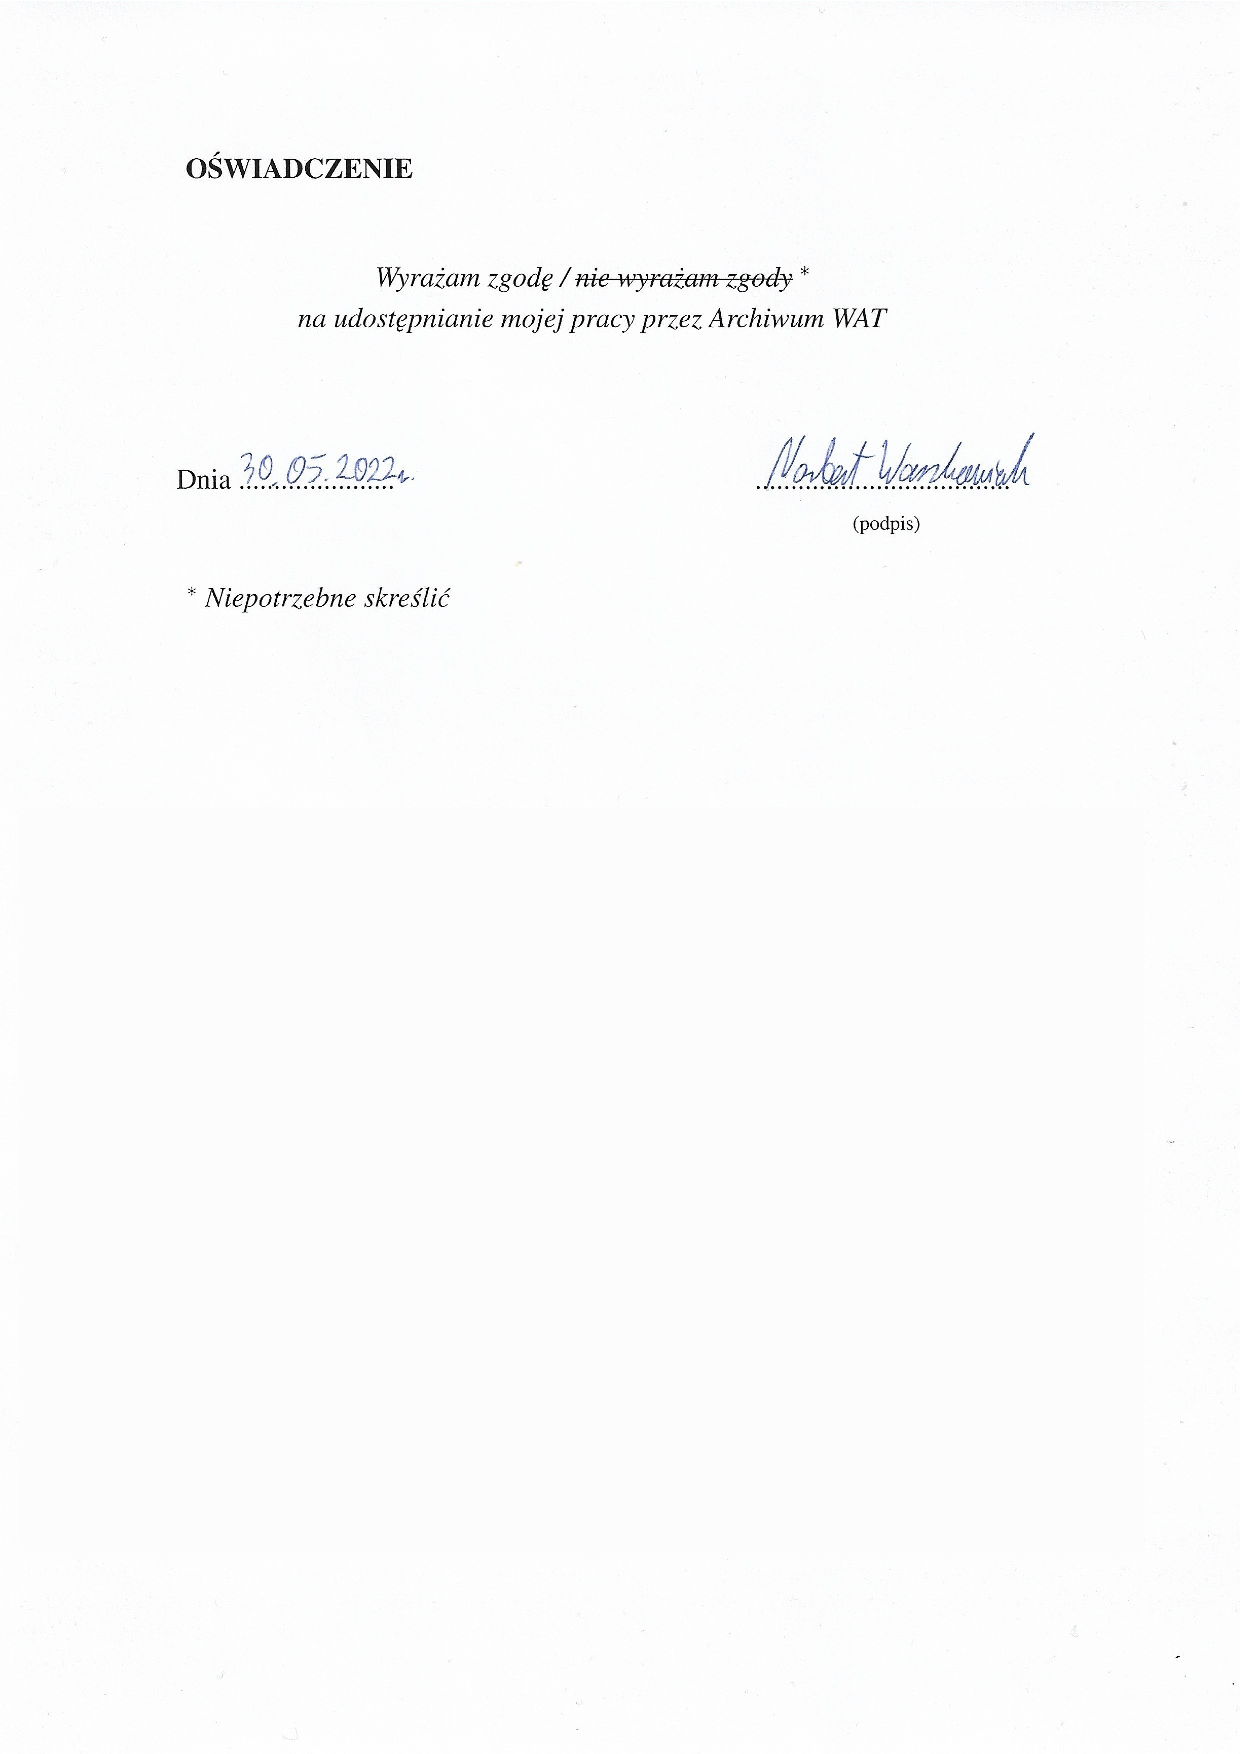
\includepdf[pages=-]{oswiadczenie.pdf}  

    \normalsize
    
    \tableofcontents
    
    \newpage
}

\defcaptionname{polish}{\refname}{Bibliografia}

\definecolor{mygray}{rgb}{0.95,0.95,0.95}

\renewcommand{\lstlistingname}{Kod.}

\lstset{
    basicstyle=\ttfamily\scriptsize,
    numbers=left,
    numberstyle=\ttfamily\scriptsize\color{black},
    numbersep=10pt,
    showspaces=false,
    breaklines=true,
    keepspaces=true,
    tabsize=2,
    xleftmargin=10pt,
    framexleftmargin=5pt,
    captionpos=tc,
    backgroundcolor=\color{mygray},
    keywordstyle=\color{black},
    inputencoding=utf8
}

\newcommand{\source}[1]{\vspace{0mm} \noindent\fontsize{10}{10}\selectfont{Źródło: {#1}}\normalsize\vspace{0mm}}

\newcommand{\TODO}[1]{
    {\large \color{red}{\underline{\textbf{TODO: #1}}}} 
}
\newcommand{\kierunek}{INFORMATYKA}
\newcommand{\stopien}{STUDIA II$^{\mathrm{o}}$} %Odpowiednie usunąć
\newcommand{\temat}{MOBILNY SYSTEM ZARZĄDZANIA I STEROWANIA BEZPILOTOWYM STATKIEM LATAJĄCYM}
\newcommand{\data}{Warszawa 2022}
\newcommand{\autor}{Norbert WASZKOWIAK}
\newcommand{\promotor}{dr inż. Michał DYK}
\newcommand{\zgoda}{TAK} %W przypadku braku zgody zakomentować tą linię
\newcommand{\specjalnosc}{SYSTEMY INFORMATYCZNE}

\newcommand{\bibTitle}[1]{``#1''}


\begin{document}

\inserttitlepage

\section*{Wstęp} 
\addcontentsline{toc}{section}{Wstęp}
    
% Zwarte wprowadzenie w temat i cele pracy z nawiązaniem do dziedziny przedmiotowej oraz rozwiązanego problemu. Uzasadnienie potrzeby i zastosowania wyników pracy. Przedstawienie układu i streszczenie zawartości rozdziałów pracy (2-3 zdania na rozdział).\\
% Zaleca się, aby tekst wstępu nie przekraczał dwóch stron.


% W pierwszym rozdziale przedstawiono definicje BSP. Następnie przyjrzano sie jej historii z uwzględnieniem tego kiedy obiekt może być zakwalifikowny jako BSP. Potem przedstawiono czołowych producntów tej technolgii i przykładowe zastosowania. Rozdział zakończono analizą możliwości dostoswywania statków do wymagań użytkownika.
\clearpage

\section{Prezentacja zagadnienia bezpilotowych statków latających oraz koncepcji ich wykorzystania}
\subsection{Definicja BSP}
W nomenklaturze związanej z domeną bezpilotowych statków latających można znaleźć wiele tożsamych terminów na określanie bezpilotowych statków latających, są to m.in.:
\begin{itemize}
  \setlength\itemsep{1mm} %TODO
  \item Bezzałogowy statek powietrzny, BSP (ang. \textit{unmanned aerial vehicle}, UAV);
  \item Bezzałogowy system powietrzny (ang. \textit{unmanned aerial system}, UAS);
  \item Samolot zdalnie sterowany (ang. \textit{remotely piloted aircraft}, RPA);
  \item Dron (ang. \textit{drone}),
\end{itemize}

Każdy z tych terminów kładzie nacisk na inną cechę, ale wszystkie nadal odnoszą się do jednego obiektu i będą w tej pracy używane zamiennie. 

Amerykański pisarz zajmujący się zagadnieniami systemów bezzałogowych i technologi obronnych,  Kelsey Artheon na łamach czasopisma \textit{Popular Science} definiuje to pojęcie następująco: "dron oznacza każdy bezzałogowy zdalnie sterowany pojazd latający, bez względu na to, czy jest to malutki, sterowany radiem helikopter-zabawka, czy też ważący 14,5 tony Global Hawk, wart 104 mln dolarów. Jeżeli coś lata i jest sterowane przez pilota z ziemi, to pasuje do potocznej definicji drona". \footnote{A. Kelsey, \textit{Flying Robots 101: Everthing You Need to Know about Drones}, Popular Science\cite{arton-kelsey}} Biorąc to pod uwagę, można zdefiniować następujące warunki do zakwalifikowania obiektu jako bezzałogowy statek powietrzny:
\begin{itemize}
  \item \textbf{bezpilotowość} - na swoim pokładzie nie posiada pilota;
  \item \textbf{dwukierunkowość} - musi mieć możliwość powrotu/wylądowania (Jest to podstawowa cecha odróżniająca drony od pocisków manewrujących); 
  \item \textbf{sterowalność} - możliwość zmiany kierunku lotu w trakcie jego wykonywania.\cite{dron-ibuk}\cite{arton-kelsey}
\end{itemize}

\subsection{Historia BSP}
Po przedstawieniu definicji BSP można przystąpić do przedstawienia historii całej tej domeny, wraz ze wskazaniem jej początku w poprawny sposób.

\subsubsection{Błędnie klasyfikowane obiekty}
Po zdefiniowaniu czym jest dron, można się zastanowić, co było pierwszym elementem spełniającym tę definicję. Autor tej pracy uważa, że kluczowym elementem umożliwiającym zakwalifikowanie obiektu jako dron jest możliwość zmiany trajektorii lotu w trakcie jego działania. W literaturze często wskazywane są dwa obiekty jako prekursory dronów, tzn. gołąb Archytasa z Tarentu i balony zawierające ładunki wybuchowe wykorzystane w konflikcie między Austrią i Wenecją w 1849 r. Pierwszy rzekomy prekursor nie umożliwia sterowania obiektem po jego wystartowaniu, więc tym samym nie jest to zgodne z przytoczonymi definicjami. Ten wynalazek można uznać za pierwszą rakietę lub robota, ale nie drona. Drugi przykład, czyli balony na gorące powietrze, również nie mogą zostać uznane za bezzałogowy statek powietrzny z tego samego powodu. Jako ciekawostkę można dodać, że pomysł Austriaków zakończył się niepowodzeniem, ponieważ wiatr zwiał balony na ich własne pozycje.\cite{dron-ibuk}. 


\begin{figure}[!ht]
  \centering
  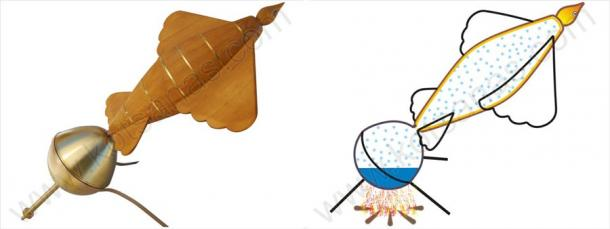
\includegraphics[width=8cm]{./Obrazy/golab.jpg}
  \caption{Latający gołąb Archytasa z Tarentu}
  \source{\myurl{https://input.niezalezna.pl//259fef5fd.jpg}}
  \end{figure}

\subsubsection{Pierwszy pełnoprawny dron}
Podczas I wojny światowej podjęto liczne próby skonstruowania bezpilotowych statków latających, ale żaden z nich nie został ukończony przed skończeniem wojny. Przykładowo \textit{Kettering Bug}, był w stanie dolecieć na odpowiednią odległość, ale jego sterowanie polegało na wyliczeniu przez operatora dokładną liczbę obrotów silnika. Mając to na uwadze, takiemu samolotowi bliżej do torpedy niż do drona. 

\begin{figure}[ht!]
  \centering
  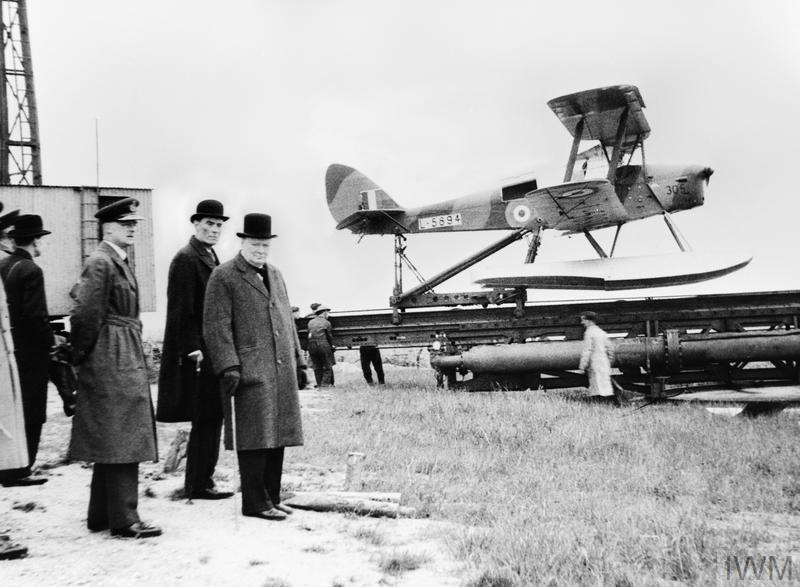
\includegraphics[width=10cm]{./Obrazy/queen-bee.jpg}
  \caption{\textit{De Havilland Queen Bee} i premier Wielkiej Brytanii Winston Churchill}
  \source{\myurl{https://www.iwm.org.uk/collections/item/object/205195356}}
  \end{figure}

W 1931 r. Królewskie Siły Powietrzne (ang. Royal Air Force) na podstawie samolotu szkolnego \textit{De Havilland DH-60T ”Tiger Moth”} opracowywały pierwszy bezpilotowy statek powietrzny \textit{DH-82B "Queen Bee"}.  Samolot ten, sterowany przez pilota za pomocą fal radiowych, miał służyć jako ruchomy cel do ćwiczeń dla obsługi dział przeciw lotniczych. Jego oficjalna prezentacja została jednak przerwana, ponieważ ówczesne systemy obrony powietrznej były tak mało skuteczne, że strzelającym skończyła się amunicja, zanim zestrzelili oni bezpilotowy samolot. Obiekt ten też spełnia wszystkie wymagania określone wcześniej przez autora, więc uznaje on go za pierwszego drona.

Równolegle w tym samym okresie, a konkretnie w 1935 r. powstał identyczny samolot dla amerykańskich odbiorców, \textit{Radioplane OQ-2}. Powstał on jako pierwotnie jako bezzałogowiec, a nie przez modyfikacje tak jak dron brytyjski, więc jego budowa bardziej odstawała od klasycznych samolotów.\cite{queen-bee}\cite{dron-ibuk}

\subsubsection{Pierwsze drony rozpoznawcze}
W bezpośrednim okresie po II wojnie światowej USA kontynuowało prace nad dronami, poprzez firmę \textit{Ryan Aeronautical Company} i ich serii dronów \textit{Firebee}, produkowanych od 1951 r. Efektem tej serii był m.in. opracowany w 1962 r. \textit{Ryan Model 147 Lightning Bug}. Był to dron rozpoznawczy, napędzany był za pomocą silnika rakietowego. Nie posiadał on wyposażenie do lądowania i startowania z ziemi, tak więc odbywała się to za pomocą spadochronu, w który był wyposażony, i jego przechwyceniu w locie przez helikopter. Sam start odbywał się z pokładu samolotu. Tak samo, jak pociski rakietowe, dron ten był umieszczany pod skrzydłem samolotu.

\begin{figure}[!ht]
  \centering
  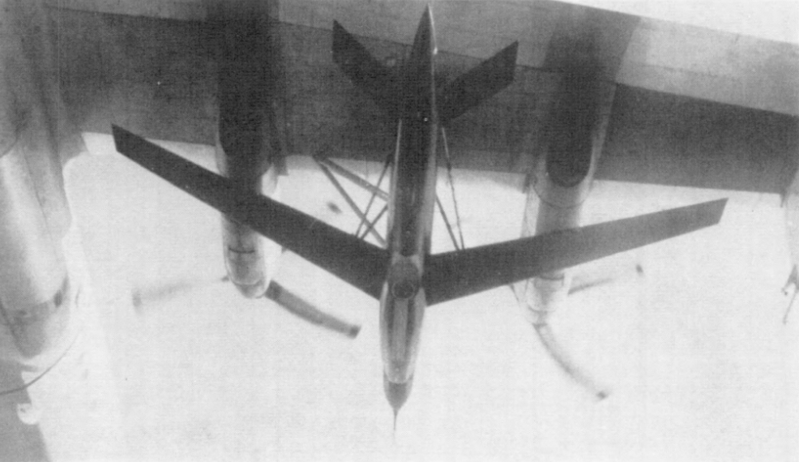
\includegraphics[width=10cm]{./Obrazy/Model_147_RPV.png}
  \caption{\textit{Ryan Model 147 Lightning Bug} umieszczony pod skrzydłem samolotu transportowego}
  \source{\myurl{https://en.wikipedia.org/wiki/File:Model_147_RPV_pictured_in_flight_under_wing_pylon_of_a_carrier_aircraft.png}}
  \end{figure}

\subsubsection{Ikona wśród BSP}
Zdecydowanie do najpopularniejszego BSP na świecie należy zaliczyć, produkowanego przez amerykańskiego producenta, \textit{General Atomics} \textit{MQ-1 Predator}. Pierwsze jego wersje nie posiadały na swoim pokładzie żadnych pocisków, ponieważ rząd USA nie byli pewni czy jest to zgodne z obowiązującym układem dotyczącym całkowitej likwidacji pocisków rakietowych średniego zasięgu (ang. \textit{Intemediate-range Nuclear Forces (INF) Traty}). Jednak wydarzenia z 11 września 2001 r. były impulsem do podjęcia decyzja o uzbrojeniu Predatorów w pociski rakietowe i skierowania ich do akcji. Umożliwiło to prowadzenie operacji militarnych bez ponoszenia strat w żołnierzach. Drony te były wykorzystywane w trakcie konfliktów w Afganistanie, Iraku czy Pakistanie. Na przestrzeni lat 2009-2021 Zjednoczona Ameryka stała się światowym liderem w używaniu dronów bojowych.\cite{dron-ibuk}\cite{predator-wiki} 


\begin{figure}[!ht]
  \centering
  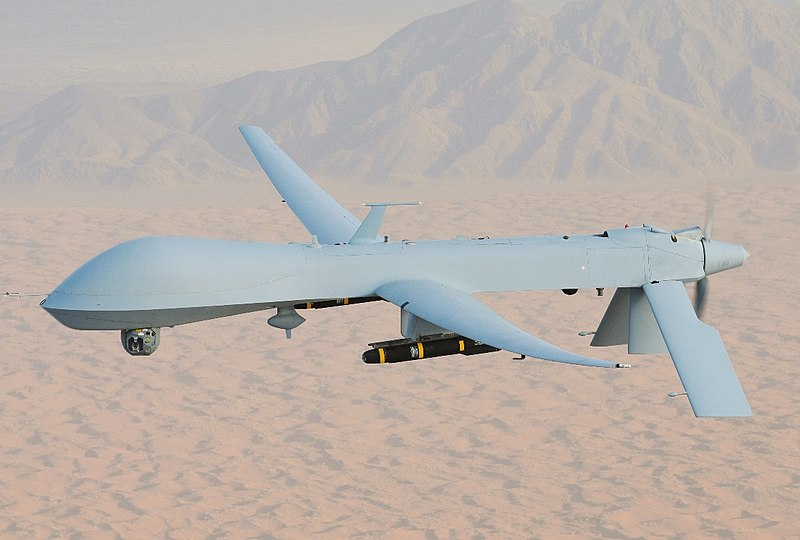
\includegraphics[width=10cm]{./Obrazy/predator.jpg}
  \caption{\textit{MQ-1 Predator}, wyposażony w rakiety \textit{AGM-114 Hellfire}}
  \source{\myurl{https://en.wikipedia.org/wiki/File:MQ-1_Predator,_armed_with_AGM-114_Hellfire_missiles.jpg}}
  \end{figure}

\subsubsection{Drony cywilne}
Trudno zaprzeczyć stwierdzeniu, że wojna przyczynia się do szybszego rozwoju, bo to właśnie rozwiązania opracowane dla armii przenoszone są często do życia codziennego. Było tak z herbatą ekspresową, jak jest i teraz z bezzałogowymi statkami powietrznym. Zmieniła się tylko ich rola, za ich pomocą nie prowadzi się działań wojennych, a nagrywa sceny do filmów, prowadzi transmisje skoków narciarskich z ciekawszej perspektywy i ratuje ludzi zagubionych w górach. Okolice obecnego roku można wskazywać jako okres największego zainteresowania tą technologią na rynku cywilnym. Początku tego okresu można próbować określać na 2013 r., czyli datę premiery pierwszej wersji, prawdopodobnie najpopularniejszej serii dronów \textit{Phantom} od obecnie najpopularniejszego producenta dronów konsumenckich \textit{DJI}.

\subsubsection{Konfilikt na Ukrainie}
W kontekście bezzałogowych statków powietrznych nie można pominąć aktualnego konfliktu zbrojnego na Ukrainie. Należy go rozpatrywać w dwóch aspektach: przewagi, która armia ukraińska uzyskuje dzięki tureckim dronom \textit{Bayraktar TB2} i wykorzystaniu dronów konsumenckich od ludności cywilnej do przeprowadzenia rozpoznania powietrznego.

Rząd ukraiński zwrócił się z prośbą do swoich obywateli o przekazanie swoich dronów na potrzeby armii. Są one wykorzystywane do bezpiecznego prowadzenie rozpoznania przez wojska ukraińskie. Dostarczają one obraz na żywo, wraz ze swoimi współrzędnymi geograficznymi. Pozwala to budować przewagę informacyjną na polu bitwy, a ten konflikt szczególnie uświadomił, jak ważna jest dzisiaj informacja na polu bitwy.\cite{fotografia-drony-ukraina}

Czytając artykuły poświęcone dronom \textit{Bayraktar TB2} w kontekście konfliktu, można odnieść wrażenie, jakby było to jedyny element budujący ich siłę. Autor nie może się z tym zgodzić, ale nie da się zaprzeczyć, że ich rola jest znacząca. Szczególnie po obejrzeniu licznych nagrań dostępnych w internecie z działań tych samolotów na wojnie. Głównym celem tej maszyny jest jednak prowadzenie rozpoznania, ale mogą być one doposażone w cztery pociski kierowane o zasięgu 8 km. Sam dron jest jedną z tańszych opcji na ryku, bo jego cena wacha się między 2-6 mln dolarów, a drony z najwyższej półki sięgają 100 mln dolarów. Rozpiętość skrzydeł tego drona to 12 metrów, a długość to 6,5 metra, co przekłada się na możliwość szybowania przez 27 godzin lub przelecenia 150 km. W dodatku wzbija się na pułap 8200 m i rozwija prędkość do 220 km/h, a wszytko to za sprawą silnika \textit{Rotax 912 iS} o mocy 100 koni mechanicznych.\cite{bayraktar-chip}\cite{bayraktar-pap}

\begin{figure}[!ht]
  \centering
  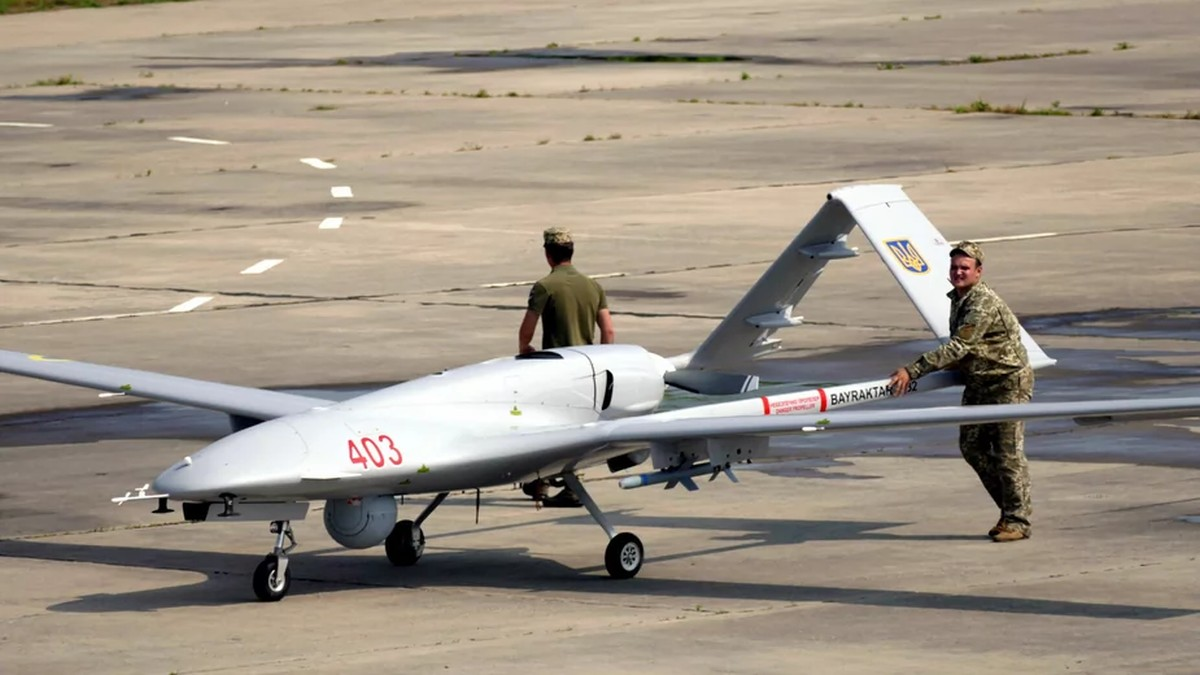
\includegraphics[width=12cm]{./Obrazy/Bayraktar_TB2_ukraina.jpg}
  \caption{Bayraktar TB2}
  \source{\myurl{https://www.instalki.pl/images/newsy/03-2022/Bayraktar_TB2_ukraina.jpg}}
  \end{figure}


\subsection{Technologia i producenci BSP}
Wymagania stawiane dronom na rynku cywilnym i militarnym znacznie się od siebie różnią, tak samo, jak konstrukcje które je spełniają. Największą różnicą jest właśnie rozmiar. Militarne BSP do realizacji swoich zadań muszą pokonywać dużo większe dystanse, przewożąc przy tym ciężkie wyposażenie. Te dwa środowiska można też uznać za hermetyczne względem siebie, rzadko następuje przejście z jedno w drugie. Większość producentów dronów wojskowych wcześniej produkowała inny sprzęt wojskowy, a cywilnych kamery czy elektryczne szybowce.

\subsubsection{Shenzhen DJI Sciences and Technologies Ltd.}
Shenzhen DJI Sciences and Technologies Ltd., znany powszechnie pod nazwą handlową DJI, jest obecnie największym producentem dronów konsumenckich. Z siedzibą w chińskiej "dolinie krzemowej" Shenzhen. Firma została założona w 2006 r., a swój pierwszy sukces odniosła w 2013 r. kiedy wpuściła na rynek pierwszy model seri dronów \textit{Phantom}. Był to BSP przeznaczony dla początkujących operatorów, a na tle konkurencji wyróżniała go łatwość obsługi. W kolejnych latach firma kontynuowała swój rozwój, a w 2015 r. wraz z wypuszczeniem trzeciej wersji jego wersji stała się ona największym producentem na świecie. W 2016 r. firma ta posiadała 50\% udziałów w światowym rynku, a rok później już 72\%. W 2020 r. było około 74\%, podczas gdy żadna inna firma w tym samym czasie nie posiadała więcej niż 5\% udziału w światowym rynku.

W 2020 r. BSP firmy DJI były wykorzystane przez Chiny do przypominania ludziom o obowiązku noszenia maseczek na twarzy w celu ograniczenia rozprzestrzeniania sie wirusa COVID-19. Z tego samego powodu w takich krajach jak Maroko czy Arabia Scytyjską drony mierzyły temperatury przemieszczającej się populacji w terenach silnie zurbanizowanych.\cite{dji-wiki}\cite{dji-market-share}

\subsubsection{Yuneec International}

Yuneec International to drugi co do wielkości producent dronów konsumenckich, pomimo że w rynku światowym posiada zaledwie 5\% udziałów. Firma ta została założona w 1999 r. i pierwotnie zajmowała się produkcją samolotów elektrycznych i szybowców. Obecnie jej siedziba znajduje się w Jiangsu w Chinach. Do swojej oferty wprowadziła pierwszego drona w 2015 r. Był on przeznaczony do fotografii. 

W 2014 r. firma została członkiem założycielem \textit{Dronecode}, organizacji non-profit prowadzonej przez \textit{Linux Foundation}, której celem jest dostarczanie otwartego oprogramowania do dronów opartego na jądrze systemu Linux. Firma \textit{Intel Corpoartion} w sierpniu 2015 r. zainwestowała 60 mln dolarów w Yuneec w zamian za 15\% udziałów. Celem inwestycji była wspólna realizacja przyszłych projektów. W tym samym miesiącu Yuneec wprowadził na rynek drona \textit{Breeze}, zdolnego do rejestrowania filmów i zdjęć w rozdzielczości UltraHD 4K. 

Również w 2015 r. firma nawiązała współprace z Ocean Alliance, organizacją zajmującą się ochroną wielorybów. Celem było stworzenie bezpieczniejszego sposobu na zbieranie danych o stanie zdrowia wielorybów. Organziacja Ocean Alliance, zamiast korzystać, tak jak dotychczas z rzutek biopsyjnych zaczęła używać do tego celów specjalnie wyposażonych dronów Yeneec.\cite{yuneec-wiki}

\subsubsection{Baykar}

W tym zestawieniu nie mogło zabraknąć producenta najpopularniejszego drona militarnego w kontekście aktualnego konfliktu zbrojnego na Ukrainie, czyli: \textit{Baykar}. Jest to prywatna firma Turecka specjalizująca się w obszarach sztucznej inteligencji, BSP i systemach \textit{Command And Control} (pl. dowodzenie i kontrola). Została ona założona w 1984 r. przez Özdemir Bayraktar i pierwotnie dostarczała części samochodowe takie jak pompy, silniki i inne. W latach dwutysięcznych firma zainteresowała się obszarem BSP, czego efektem było wyprodukowanie \textit{Bayraktar Mini UAV}. Był to pierwszy dron w całości wyprodukowany z kapitału krajowego Turcji i w 2007 r. znalazł się na wyposażeniu Tureckich Sił Zbrojnych. Rozpoczęcie prac badawczo-rozwojowych przyczyniło się do produkcji pionierskich i zaawansowanych systemów. Portfolio firmy obejmuje również latający samochód, nazwany \textit{Cezeri}, który w trakcie testów w Stambule we wrześniu 2020 r. Wzniósł się na wysokość 10 m.\cite{baykar-wiki}

\begin{figure}[!h]
  \centering
  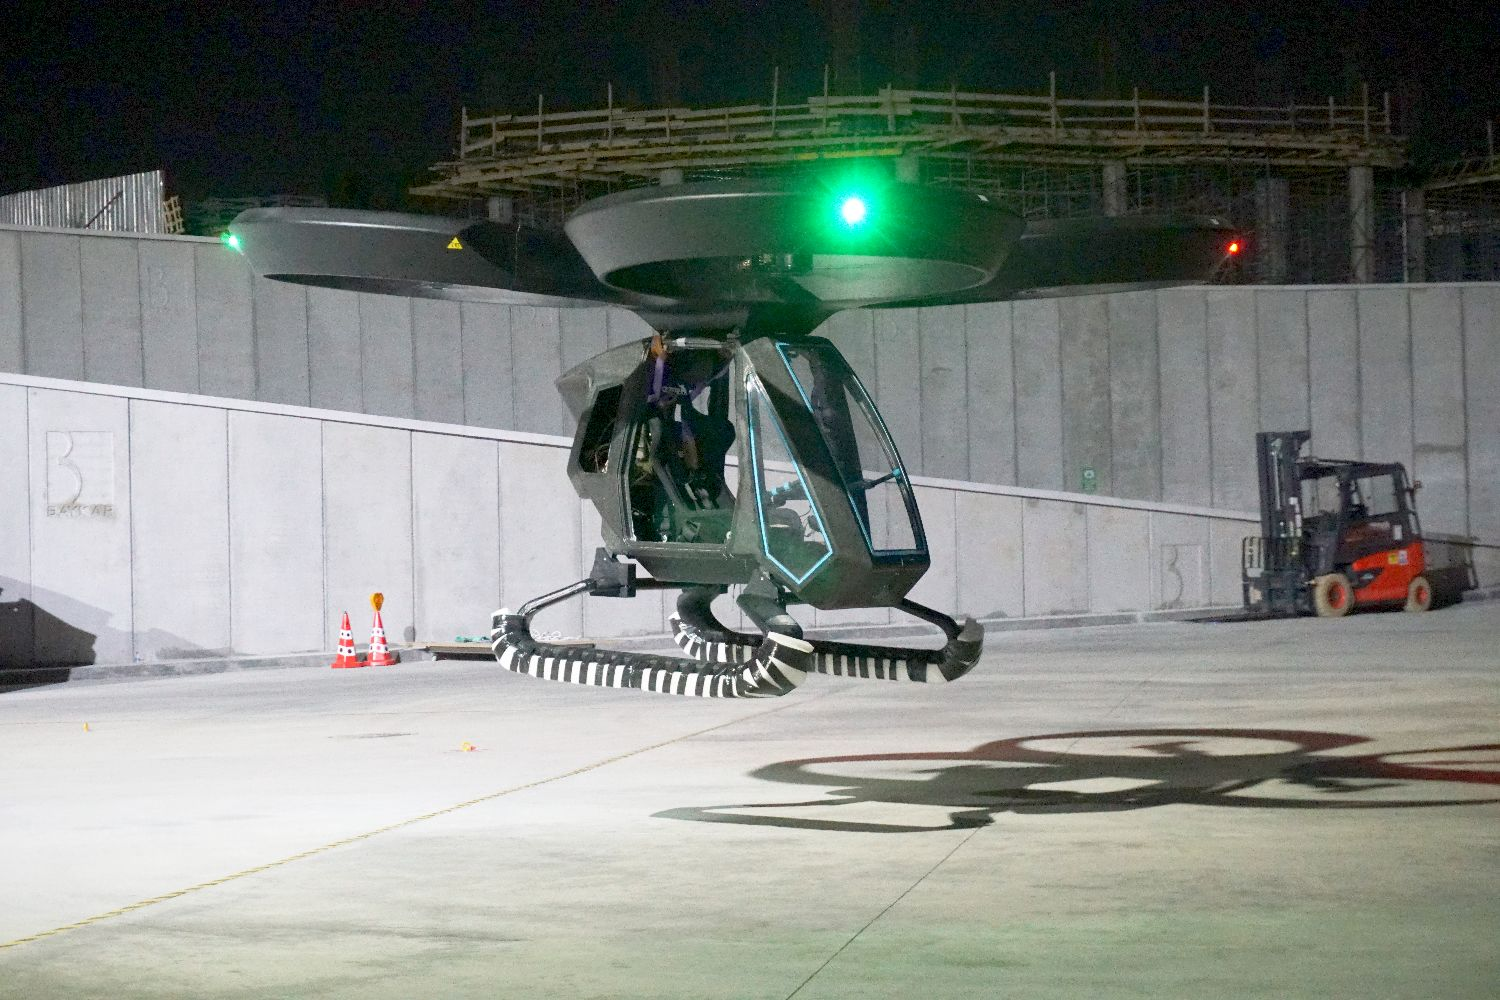
\includegraphics[width=12cm]{./Obrazy/cezarei.jpg}
  \caption{Dron osobowy Cezarei w trakcie testów w Stambule}
  \source{\myurl{https://www.savunmahaber.com/en/wp-content/uploads/2020/09/CEZERI-UCAN-ARABA-26.jpg}}
  \end{figure}

\subsubsection{General Atomics}
\textit{General Dynamics Corporation} to amerykańska korporacja założona w 1952 r., z siedzibą w Reston, w stanie Wirginia. Do 1990 r. dostarczała on czołgi, rakiety, pociski, łodzie podwodne, okręty wojenne, myśliwce i elektronikę dla wszystkich rodzajów wojsk. Na początku lat 90tych sprzedała całe swoje portfolio, z wyjątkiem działalności związanej z pojazdami wojskowymi i okrętami podwodnymi.

Korporacja ta jest właścicielem \textit{General Atomics Aeronautical Systems}, która zajmuje się produkcją systemów radiowych i bezzałogowych statków powietrznych, w tym rewolucyjnego kiedyś drona wojskowego \textit{Predator}. Seria tych dronów jest nadal rozwijana, a poszczególne konstrukcje są do siebie bardzo zbliżone.\cite{gd-about}\cite{wiki-gaas}

\subsection{Zastosowania BSP}
Bezpilotowe statki latające znalazły szereg zastosowań, pierwotnie były wykorzystywane głównie w obszarze militarnym, dopiero później dostrzeżono w nich potencjał również w środowisku cywilnym. Ponieważ kontekst militarny został już dość szczegółowo przedstawiony, w poniższym tekście przyłożono większą uwagę do ich cywilnych zastosowań.

\subsubsection{Militarne zastosowania BSP}
Bezzałogowe statki powietrzne w kontekście militarnym można dokonać podziału na następujące kategorie: 
\begin{itemize}
  \item \textbf{bojowe} - przenoszące i używające środki bojowe/ środki rażenia, np. \textit{Bayraktar TB2};
  \item \textbf{amunicja krążąca} - umożliwiające wykrywanie, rozpoznanie oraz atak na wyznaczony cel poprzez autodestrukcje, np. \textit{WB Electronics Warmate};
  \item \textbf{operacyjno-rozpoznawcze} - realizjące rozpoznawanie oraz śledzenie obiektu/celu, a także monitorowanie i kontrole obszaru zainteresowania, np. granic lub strefy przybrzeżnej. Przykładem takiego drona jest \textit{Lockheed Martin RQ-170 Sentinel};
  \item \textbf{wsparcia}: umożliwiające ewakuacje lub dostawę amunicji, wyposażenia, środków medycznych i żywności do wysuniętych stanowisk wojsk własnych, np. \textit{Kaman KARGO UAV} \cite{konkurs-mon}
\end{itemize}

\subsubsection{Cywilne zastosowania BSP}
Wymienienie wszystkich cywilnych rozwiązań jest trudne, ponieważ rynek ten znajduje co chwilę kolejne zastosowania dronów. Poniżej przedstawiono parę wyselekcjonowanych interesujących rozwiązań.

\myparagraph{Transport medyczny}
W czerwcu 2022 r. Polska Agencja Żeglugi Powietrznej wydała zgodę na wykonywanie regularnych długodystansowych lotów BSP. Realizować będzie je firma transportowa na rzecz systemu opieki zdrowotnej. Połączenie obejmie dwie trasy Warszawa-Pułtusk i Warszawa-Sochaczew. Przewidywana częstotliwość lotów to ok. 7 w tą i z powrotem w ciągu dnia. Obie te trasy mają długość 60 km i odbywają się na wysokości 100 m. Sam samolot posiada systemy wizyjne, które będą korygowały lot w przypadku wystąpienia przeszkód na jego trasie przelotu. Takie połączenie zapewni szybki transport np. narządów do przeszczepu co może przyczynić się do uratowania komuś życia. \cite{pansa-lot-medyczny}

\begin{figure}[!h]
  \centering
  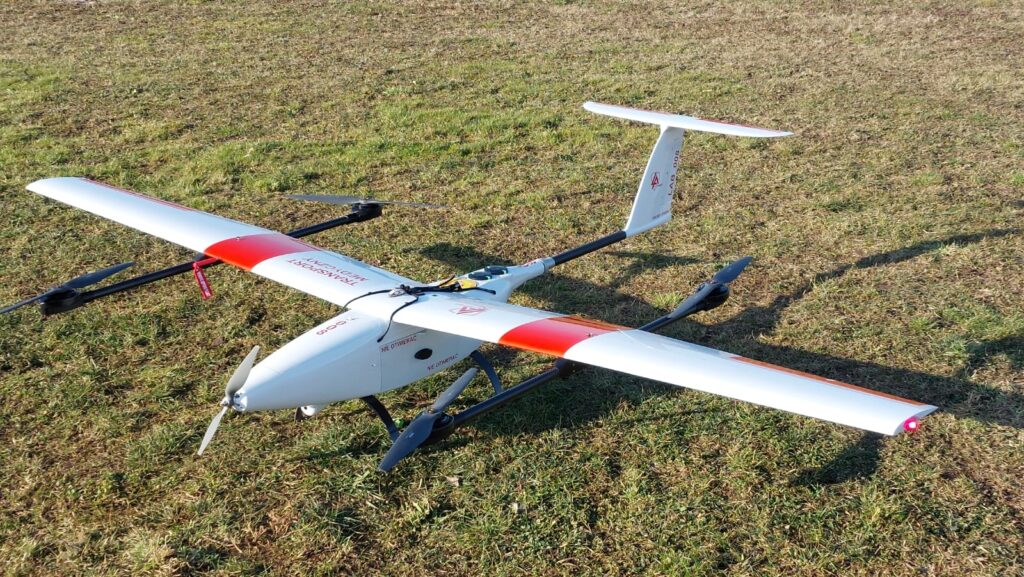
\includegraphics[width=10cm]{./Obrazy/Farada_G1.jpg}
  \caption{Dron \textit{Farada G1}, za pomocą którego będzie obywał się transport medyczny w okolicach Warszawy}
  \source{\myurl{https://www.pansa.pl/wp-content/uploads/2022/02/IMG-20220213-WA0001-1024x577.jpg}}
  \end{figure}

\myparagraph{Ratownictwo}
Drony powietrzne pomagają również w ratowaniu ludzkiego życia, szczególnie w górach. W styczniu 2022 r. ze względu na trudne warunki atmosferyczne ratownicy TOPR nie mogli udzielić pomocy dwóm turystą, którzy nie byli w stanie zejść z góry. Za pomocą drona dostarczono im koce i ogrzewacze, co pozwoliło im przetrwać noc. Kolejnego dnia, gdy pogoda uległa poprawie ratownicy dotarli do poszkodowanych i ich sprowadzili w bezpieczny sposób.\cite{topr-dron}

Również na dalekim zachodzie można znaleźć przykłady ratowania życia z użyciem BSP, a konkretnie w Północnej Kalifornii. Właśnie tam, w lesie, zgubił się młody myśliwy. Służby za pomocą drona zlokalizowali jego lokalizacje, a następnie wysłali tam strażników, którzy z jego pomocą wyprowadzili zagubionego.\cite{bbc-drone-rescue} 

Są cztery powody, dla którego BSP dobrze odnajdują się w ratownictwie.
\begin{itemize}
  \item \textbf{Czas reakcji} - są opcją bardzo szybkiego reagowania, czas potrzebny na przygotowania do startu jest minimalny;
  \item \textbf{Szybkie przeszukiwania} - mogą przeszukac trudny teren w dużo szybszym czasie niż człowiek pieszo;
  \item \textbf{Komunikacja} - mogą koumunikować sie z poszkodowanymi za pomocą głosnika i mikrofonu;
  \item \textbf{Lokalizacja} - są w stanie przekazywać na żywo do operatora swoją aktualną lokalzacje, co w przypadku ratowania i poszukiwania osób może znacznie minimalizować czas poszukiwania i ewakuacji. \cite{snowbrains-drone}
\end{itemize}

\myparagraph{Kinematografia i produkcja filmowa}
Jednym z pierwszych filmów, które przywoływane jako przykład dobrego wykorzystania dronów jest \textit{Skyfall} z 2012 r., a konkretnie scena pościgu motorem przez Jamesa Bonda złoczyńców po dachach w Istambule. BSP dały kinematografii wyjątkową przewagę nad tradycyjnymi metodami filmowania. Mają większy zasięg niż żuraw i są też bardziej zwinne niż helikopter. Reżyserzy dzięki temu mogą wykonywać bardziej ryzykowne, prawdziwie akrobatyczne ujęcia, które gdyby nie drony musiałyby być wytworzone na komputerze. Nie można zapomnieć, że BSP są przede wszystkim tańsze w zakupie i utrzymaniu niż np. helikoptery.\cite{washingtonpost-drone-movie}

Przykładem gdzie wcześniej nie było możliwe nagrywanie ujęć filmowych, są erupcje wulkanów. Takie loty wiązały się z dużym niebezpieczeństwem, a drony są dużo tańsze i nie posiadają na swoim pokładzie załogi, tak więc operatorzy mogą pokusić się o takie ryzyko. Takie nagranie wykonał znany youtuber Joey Helms, który postanowił uwiecznić z bliska rzekę lawy wyrzucaną przez wulkan Fagradalsfjall na Islandii. W trakcie nagrywania erupcja lewy w pewnym momencie sięgnęła jego statku. Youtuber bezpowrotnie stracił swój statek. Ujęcie, które zostało zachowane, jest bardzo emocjonujące, więc prawdopodobnie było to warte swojej ceny.\cite{dron-lawa-pogoda}

\myparagraph{Transport towarów}

W 2013 r. Jeff Bezos ogłosił koncepcje, która miała zrewolucjonizować transport towarów. Autonomiczne drony powietrzne miały dostarczać paczki Amazonu w 30 minut pod drzwi odbiorcy. Mogły one zaoferować konsumentom dostawę żywności, leków czy innych lżejszych przedmiotów, bez spalania paliw kopalnianych i czekania. Niestety jednemu z najbogatszych ludzi na świecie nie udało się tego osiągnąć. Tak samo, jak firmie \textit{Zipline}, która miała dostarczać leki w Rwandzie i projektowi Google \textit{Wing}, który miał zapewniać burito głodnym studentom. Na świecie istnieje duża presja na wprowadzenie takiego rozwiązania. W 2021 r. Amazon zwolnił większość pracowników odpowiedzialnych za rozwój wspominanego projektu, uzasadnił to błędem w zarządzaniu i panującym chaosem. W tym samym roku DHL również ogłosił zakończenie swojego identycznego projekty. Było to 8 lat po tym, gdy ich dron pierwszy raz wbił się w powietrze.Koszty transportu towaru między centrum dystrybucji a klientem końcowym to 40\% całkowitego kosztu, a konsumenci oczekują szybkiej taniej i ekologicznej dostawy. Wszystkie te potrzeby mogłyby zaspokoić dostawy dronami.

Jest parę czynników, które mogły wpłynąć na wstrzymanie masowych dostaw towarów dronami. Głownym z nich jest prawodopodobnie ograniczenie stref lotów BSP. Osoby zarządzające państwami i miastami na bieżąco wprowadzają regulacje w tej dynamicznie rozwijającej sie domenie. Wprowadzone zostały m.in. sterefy wyłączone dla dronów, które mają zapewnić bezpieczeństwo wokół miejsc wymagających specjalnej ochorny. Są to najczęściej okolice lotnisk i jednostek wojskowych. Takie strefy mocno ograniczają dostawy towarów dronami.\cite{drone-transport}


\begin{figure}[!ht]
  \centering
  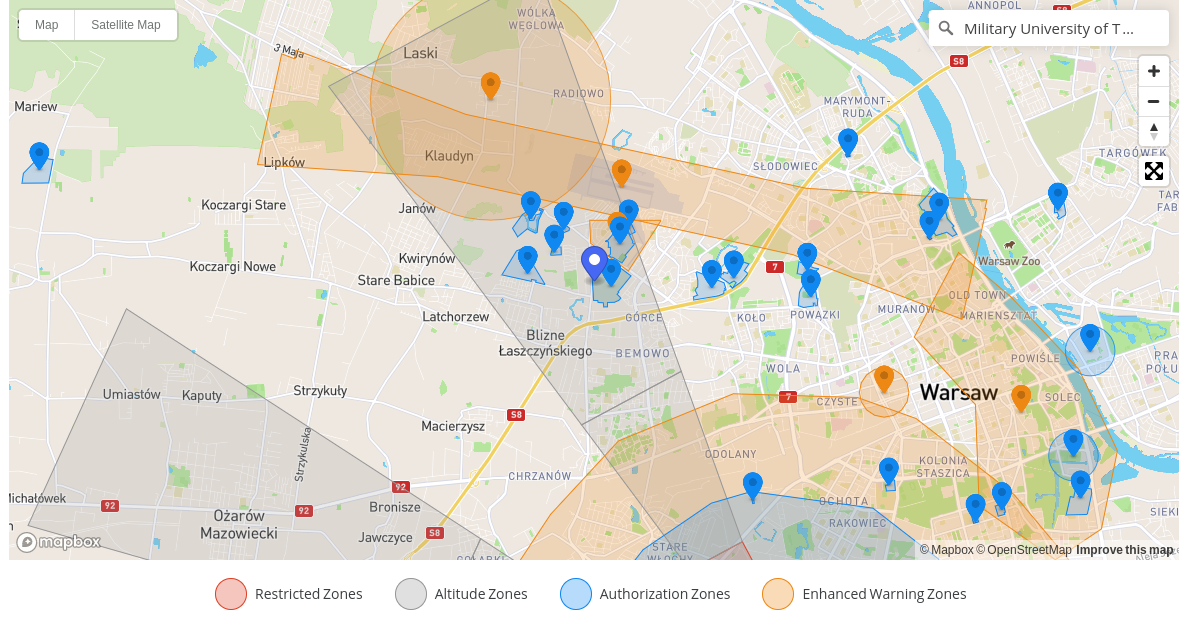
\includegraphics[width=16cm]{./Obrazy/no2.png}
  \caption{Strefy wyłączone dla dronów w okolicach Warszawy}
  \source{\myurl{https://www.dji.com/pl/flysafe/geo-map}}
  \end{figure}
  
Mimo wszystko taki transport jest jednak nadal możliwy, ale nie na masową skalę. W Sosnowcu od 2021 r. realizowany jest projekt, w którym drony będą świadczyły usługi transportu m.in. pilnych przesyłek medycznych. Odbiór i nadawanie będzie odbywało się w stacjach dokujących, które będą automatycznie ładowały i zdejmowały ładunek z drona. Wykorzystanie takich punktów umożliwia ustawienie stałej trasy lotów, co zdejmuje duża część odpowiedzialności z uczestników projektu, dlatego też w przyszłości można spodziewać się większej ilości tego typu rozwiązań.\cite{sosnowiec-drone}


\subsection{Dostosowywanie BSP do wymagań użytkownika}
Na rynku znajduje się duża ilość dostępnych komponentów, z których można łatwo zbudować własne bezzałogowe statki powietrzne. Najwięcej odpowiedzialności z konstruktora zdejmują gotowe kontrolery lotu, np. \textit{pixhawk}, na którym można zainstalować otwarte oprogramowanie \textit{ArduPilot}. Pozwala to zachować duża ilość zasobów, bo cała logika lotu jest praktycznie \textit{out-of-the-box} Przykładowy zestaw elementów potrzebnych do zbudowania własnego drona to::
\begin{itemize}
  \setlength\itemsep{1mm} %TODO
  \item rama,
  \item silnik,
  \item elektroniczny kontroler prędkości,
  \item śmigła,
  \item załącza,
  \item rozdzielnia zasilająca,
  \item baterie,
  \item monitoring baterii,
  \item mata montażowa,
  \item kontroler,
  \item odbiornik RC,
  \item kamera,
  \item karata pamięci SD.\cite{how-to-build-drone}
\end{itemize}

\begin{figure}[!ht]
  \centering
  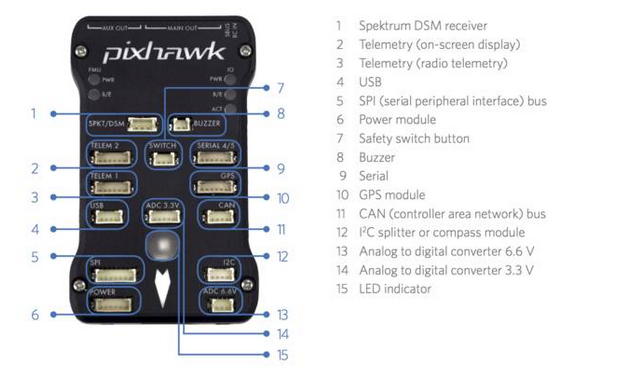
\includegraphics[width=12cm]{./Obrazy/pixhawk.png}
  \caption{Kontroler lotu Pixhawk}
  \source{\myurl{https://ardupilot.org/plane/_images/Pixhawk_with_legend.jpg}}
  \end{figure}

Budowa własnego drona jest jak najbardziej możliwa, bez wymagania specjalistycznej wiedzy, ale nadal to potrzeba na to dużo ilości zasobów, szczególnie czasu, dlatego warto przyjrzeć się gotowym rozwiązaniom dostarczanym przez producentów i to jak bardzo można je dostosowywać. Firma DJI udostępnia do swoich produktów SDK, czyli bibliotekę, za pomocą której można zaprogramować działanie naszego drona. Dodatkowo producent dla wybranych statków przygotował szereg rozszerzeń, które pomogą dostosować wyposażenie do naszych wymagań. Przykładowo dla \textit{Mavic 2 Enterprise Advaced} dostępne są:
\begin{itemize}
  \item \textbf{głośnik} - który umożliwia komunikacje z drona, np. w czasie sytuacji alarmowych do ludności znajdującej sie na ziemi
  \item \textbf{dodatkowe oświetlenie} - w przypadku wystąpienie niekorzystnych warunków atmosferycznych lub lotów w nocy
  \item \textbf{moduł RTK} - który umożliwia osiągnięcie dokładności lokalizacji na poziomie jednego centymetra
\end{itemize}
Dodatkowo dla innych modeli dostępne są wyspecjalizowane kamery np. do skanu obiektów w 3D czy podglądu w podczerwieni.

\newpage 
\section{Przegląd i prezentacja technologii mobilnych z uwzględnieniem aspektów tworzenia aplikacji i komunikacji M2M}
W tym zdefiniowano cel i wymagania stawiane technologią M2M. Następnie przedstaw przedstawiono przykładowe technologie ze szczególnym uwzględnieniem komunikacji pomiędzy bezzałogowym statkiem powietrznym a kontrolerem. Rozdział zakończono analizą interfejsu API umożliwiającego kontrolowanie drona.

\subsection{Komunikacja M2M}
Komunikacja M2M (machine-to-machine) to kategoria technologii, która umożliwia wymianę informacje pomiędzy urządzeniami w sieci bez jakikolwiek ingerencji ludzi. Obiekty pracujące w tej sieci charakteryzują się mniejszą lub większą autonomią. Wspierana jest ona często szeroko pojętą sztuczną inteligencją, ze szczególnym uwzględnieniem technik uczenia maszynowego. Ta komunikacja jest podstawą istnienia IoT.\cite{m2m-web}

\subsubsection{Cel}
Głównym celem M2M jest autonomiczna komunikacji pomiędzy maszynami, a jej obecnie najczęstszym zastosowaniem jest przenoszenie danych z sensorów do sieci. Obecnie operatorzy coraz częściej rozbudowują swoją infrastrukturę o węzły zgodnie z tą kategorią technologii. Dzięki temu koszty utrzymania całego systemu są znacznie zredukowane. Składają się na niego następujące elementy:
\begin{itemize}
  \item łącze do przesyłu danych, np. WiFi, GSM
  \item sensory, np. czujnik temperatury, kamera
  \item oprogramowanie, które automatyzuje procesy komunikacyjne, np. przeszukiwanie ścieżki routingu
\end{itemize}
Celem telemetrii jest automatyczny pomiar wielkości fizycznej przez odpowiednie sensory. Wartość pomiaru jest przesyłana do miejsca, zwykle odległego, w którym jest dalej przetwarzana. Na początku do tego celu były wykorzystywane linie telefoniczne, a następnie radiowe. Rozwój technologii, a w tym łączności bezprzewodowej sprawił, że poszerzyła się rola wykorzystywania telemetrii w nauce, inżynierii i produkcji. Dzisiaj jest ona używana także w życiu codziennym, w jednostkach grzewczych, miernikach elektrycznych i wszelkich urządzeń podłączonych do internetu. Jej rozwój jest ściśle powiązany z komunikacją M2M.\cite{m2m-web}

\subsubsection{Wymagania}
Według Europejskiego Instytutu Norm Telekomunikacyjnych (ETSI) komunikacja M2M musi spełniać następujące wymagania:
\begin{itemize}
  \item \textbf{Skalowalność}: w miarę dołączania kolejnych urządzeń do systemu system nadal musi funkcjonować;
  \item \textbf{Anonimowość}: w związku z wymaganiami prawnymi, na każde żądanie system musi umożliwiać ukrywanie tożsamości urządzenia;
  \item \textbf{Logowanie}: ważne wydarzenia w systemie, takie jak: pojawienie się błędnych informacji czy nieudane próby instalacji, muszą być zarejestrowane, a rejestry te muszą być dostępne na żądanie;
  \item \textbf{Zasady komunikacji między aplikacjami}: aplikacje w systemie powinny mieć możliwość komunikowania się. W szczególności bramki i urządzenia końcowe komunikujące się za pomocą technologi SMS czy Ethernet powinny komunikować się za pomocą połączenia P2P (peer-to-peer);
  \item \textbf{Metody dystrybucji}: w ramach systemu powinny być dostarczane metody dystrybucji takie jak: \emph{unicast}, \emph{multicast}, \emph{broadcast} i \emph{annycast}, a wszędzie gdzie to możliwe metoda \emph{broadcast} powinna być zastąpiona za pomocą \emph{multicast}, tak aby zminimalizować obciążenie sieci;
  \item \textbf{Harmonogram przesyłania komunikatów}: dostęp do sieci powinien być kontrolowany, tak samo, jak harmonogram przesyłania komunikatów. Sam system powinien również uwzględniać obciążenia aplikacji M2M w harmonogramie przesyłania wiadomości;
  \item \textbf{Wybór ścieżek komunikacyjnych}: ścieżki w systemie powinny zapewniać optymalizacje bazującą na: awariach transmisji, kosztu i opóźnieniach, w momencie, gdy istnieją inne ścieżki do punktu docelowego. \cite{m2m-web}
\end{itemize}

\subsection{Technologie komunikacji M2M}
Poprawnym stwierdzeniem będzie, że obecnie znajdujmy się w epoce połączonych ze sobą obiektów. IoT (Internet of Things) zdobywa aktualnie coraz więcej uwagi nie mal w każdej domenie, a szczególnie w takich jak biznes, elektronika konsumencka, przemysł czy transport. Niemal każdy obiekt elektryczny w dzisiejszym świecie jest ze sobą połączony w ten czy inny sposób. Siedząc w biurze, za pomocą dostarczanych aplikacji, możemy kontrolować drzwi, bramę garażową, czajnik elektryczny czy rolety okienne w naszym domu. Z kolei w mieście kontrolujemy kamery i oświetlenie, a wszystko to z odległych lokacji. IoT odgrywa w tym ważną rolę, ponieważ to ono umożliwia łączenie przeróżnych obiektów, za pomocą sieci połączeń i wymianę danych między nimi.\cite{LoRa-article}


\newpage
\subsubsection{Ogólna klasyfikacja technolgi M2M}
Poniżej przedstawiono ogólne porównanie technologi komunikacyjnych M2M.

\begin{table}[!htbp]
  \resizebox{\textwidth}{!}{%
  \begin{tabular}{|l|l|l|l|}
  \hline
  \textbf{}            & \begin{tabular}[c]{@{}l@{}}\textbf{Local Area Network}\\ Komunikacja krótko \\ dystansowa\end{tabular}            & \begin{tabular}[c]{@{}l@{}}\textbf{Low Power Wide Area}\\ Intenet Of Things\end{tabular}            & \begin{tabular}[c]{@{}l@{}}\textbf{Celluar Network}\\ Tradycyjne M2M\end{tabular}                               \\ \hline
  \textbf{Użycie}      & 40\%                                                                                                              & 45\%                                                                                                & 15\%                                                                                                            \\ \hline
  \textbf{Zalety}      & \begin{tabular}[c]{@{}l@{}}- Dobrze ugruntowana norma\\ - W budynkach\end{tabular}                                & \begin{tabular}[c]{@{}l@{}}- Niskie zużycie energi\\ - Niskie koszty\\ - Pozycjonowanie\end{tabular} & \begin{tabular}[c]{@{}l@{}}- Istniejące pokrycie znacznego \\ obszaru\\ - Duża prędkość transmisji\end{tabular} \\ \hline
  \textbf{Wady}        & \begin{tabular}[c]{@{}l@{}}- Wysokie zużycie energi \\ elektrycznej\\ - Duży koszt sieci i zależności\end{tabular} & \begin{tabular}[c]{@{}l@{}}- Niska prędkość transmisji\\ - Wschodzący standard\end{tabular}         & \begin{tabular}[c]{@{}l@{}}- Wysoki koszt posiadania\\ - Mała autonomia\end{tabular}                            \\ \hline
  \textbf{Technologia} & Bluetooth, WiFi                                                                                                   & LoRa                                                                                                & GSM, 3G, 4G, 5G                                                                                                 \\ \hline
  \end{tabular}%
  }
  \caption{Porównanie rodzajów technologi M2M.\cite{LoRa-article}}
\end{table}


\subsubsection{LoRa}
Komunikacja w aplikacjach IoT jest dzisiaj wykonywana w przeróżnych technologiach, a każda z nich ma swoje zalety, funkcje, a przez to też przeznaczenie. Żadna z tych technologi nie może pokryć całego zapotrzebowania świata IoT, ponieważ wszystkie one posiadają cechy, które czynią je odpowiednie dla postawionego konkretnego zadania.

LoRa (Long Range) to nowa technologia połączeń bezprzewodowych w świecie IoT. Ostatnio znacznie ewoluowała i zyskała szczególną popularność w urządzeniach z ograniczoną pojemnością elektryczną, umożliwiając systemom wbudowanym przesyłanie małej ilości danych na dużych dystansach w krótkich interwałach czasowych.

WiFi to najpopularniejsza technologia komunikacji bezprzewodowej, która jest już rozwijana przez wiele lat. W kontekście IoT wykorzystywana jest przede wszystkim do komunikacji na dużych
odległościach. Na krótkie dystanse lepiej pasują do tego takie protokoły jak Bluetooth czy ZigBee. We wszystkich z nich największą wadą jest duże zużycie energii elektrycznej. Technologia Lora zapewnia bezpieczne, mobilne dwukierunkowe połączenie o niskim koszcie elektrycznym. Wykorzystywane jest ono w IoT, szczególnie w domenie smart city, czy nawet ogólnej komunikacji M2M. LoRa zalicza się do LPWA(Low Power Wide Area), czyli rodzaju bezprzewodowej rozległej sieci telekomunikacyjnej, stworzonej w celu umożliwienia komunikacji na duże odległości przy niskiej przepływności i niskim poborze energii. \cite{LPWA-wiki} W tego typu komunikacji wyróżnia się LoRa ze względu na jej:
\begin{itemize}
  \setlength\itemsep{0.8mm} %TODO
  \item długodystansowość;
  \item dwukierunkowość;
  \item wysoką pojemność węzłów w sieci;
  \item długość życia na baterii;
  \item odporność interfejsów;
  \item bezpieczeństwo i efektywność sieci. \cite{LoRa-article}
\end{itemize}


\myparagraph{Cechy}
Technologie tą wyróżniają następujące cechy:
\begin{itemize}
  \setlength\itemsep{1mm} %TODO
  \item Pojedyncza bramka może pokryć obszar aż $100km^2$;
  \item Oferuje ona podwójne szyfrowanie AES;
  \item Bazuje na technologi CSS (widmo rozproszone Chrip), które umożliwia śledzenie obiektów i jest odporne na zanikanie sygnałów;
  \item Topologia gwiazdy eliminuje zanikanie danych przez urządzenia pośrednie, co przyczynia się do zmniejszenia poboru mocy. \cite{LoRa-article}
\end{itemize}


\myparagraph{Ograniczenie przepustowości}
W sieci LoRa wszystkie klasy ramek wymagają potwierdzenia. Wiąże się z tym, że po każdym potwierdzeniu ramki przez urządzenie końcowe w dowolnym oknie czasowym następuje okres wyłączenia, w celu zachowanie zgodności z przepisami dotyczącymi cyklu pracy. W związku z tym, aby uniknąć wyczerpania limitu pojemności przez sieć i urządzenia końcowe, muszą one ograniczyć liczbę potwierdzeń. Również w podsieciach LoRa po przesłaniu danych następuje okres wyłączenia, w którym na danym kanale nie są wysyłane żadne dane. Te dwa okresy, tzn. okres wysyłania danych i wstrzymania transmisji stanowi cykl pracy. Cały ten mechanizm przyczynia się do ograniczenia przepustowości sieci.\cite{LoRa-article}

\subsubsection{Narowband IoT}
Wraz z rozwojem świata IoT zyskała również technologia Narowband IoT (NB-IoT). Wykorzystywana jest ona przede wszystkim przy komunikacji komórkowej dla zdalnych pomiarów w całej Europie. Jest to technologia dostępu radiowego. Używa ona ponownie kompnentów stworzonych przez jej poprzednika LTE, aby umożliwić jej działa na licencjonowanej częstotliwości. Może ona również działać w trybie autonomicznym. Tak jak sama nazwa wskazuje, cały system działa w wąskim spektrum częstotliwości, bo tylko w 200kHz, co wprowadza elastyczność zastosowań dzięki minimalnym wymaganiom częstotliwości, w porównaniu do jej poprzednika LTE. Cała szerokość 200kHz została podzielona na kanały po 3.75 kHz lub 15 kHz, co umożliwia połączenie w bardzo wysoką prędkość nadawania, a także daleki zasięg połącznia. \cite{nbiot-article}  

\subsubsection{NB-IoT vs Lora}

\begin{table}[!htbp]
  \resizebox{\textwidth}{!}{%
  \begin{tabular}{|l|c|c|}
  \hline
  \textbf{Parametr}                                                                     & \textbf{LoRa}               & \textbf{NB-IoT}       \\ \hline
  \textbf{Pasmo}                                                                        & 125 kHz                     & 180 kHz               \\ \hline
  \textbf{Pokrycie}                                                                     & 165 dB                      & 164 dB                \\ \hline
  \textbf{Żywotność baterii}                                                            & 15+ lat                     & 10+ lat               \\ \hline
  \textbf{\begin{tabular}[c]{@{}l@{}}Maksymalne natężenie \\ elektryczne\end{tabular}}  & 32 mA                       & 120 mA                \\ \hline
  \textbf{\begin{tabular}[c]{@{}l@{}}Spoczynkowe natężenie \\ elektryczne\end{tabular}} & 1 µA                        & 5 µA                  \\ \hline
  \textbf{Przepustowość}                                                                & 50 Kbps                     & 60 Kbps               \\ \hline
  \textbf{Opóźnienie}                                                                   & Zależne od klasy urządzenia & 10 s                  \\ \hline
  \textbf{Bezpieczeństwo}                                                               & AES 128 bit                 & 3GPP (128 to 256 bit) \\ \hline
  \textbf{Geolokalizacja}                                                               & Tak (TDOA)                  & Tak (In 3GPP Rel 14)  \\ \hline
  \textbf{Jakość/cena}                                                                  & Wysoka                      & Średnia                \\ \hline
  \end{tabular}%
  }
  \caption{Porównanie technologi LoRa i NB-IoT \cite{NB-IoT_vs_Lora}}
  \end{table}

  
Zarówno LoRa, jak i NB-IoT należą do wspomnianej wcześniej technologi LPWAN. Podstawowa różnice pomiędzy tymi dwoma technologiami można dostrzec w zużyciu baterii, prędkości transmisji i opóźnień.

\subsection{Komunikacja bezprzewodowa w dronach konsumenckich}
Przeglądając katalog największego producenta dronów konsumenckich DJI, można wyróżnić tylko 3 technologie komunikacji bezprzewodowej: wzomocnione WiFi (ang. enhanced WiFi), Lightbridge, OcuSync.

\subsubsection{WiFi}
WiFi nie zostało wprowadzone ściśle do komunikacji bezprzewodowej statków powietrznych, ale odnajduje się w tym całkiem dobrze. Jest ona wykorzystywana głównie w bardziej budżetowych wersjach dronów, ze względu na możliwość skorzystanie przez producenta z posiadanej przez użytkownika infrastruktury (smartfonów), czy niskiej ceny komponentów.

Przykładowo dron \textit{DJI Tello}, który jest najtańszą opcją dostępną od producenta DJI, przeznaczoną głównie do nauki latania i programowania, również przez najmłodszych pasjonatów. Nie posiada on w zestawie dedykowanego kontrolera, poniewąż odbywa się ono za pomocą aplikacji na smartfona, która łączy się z dronem za pomocą WiFi tak jak do punktu dostępowego z internetem. Zasięg takiego połączenia według producenta to 100 m.\cite{dji-store}


\begin{figure}[!htbp]
  \centering
  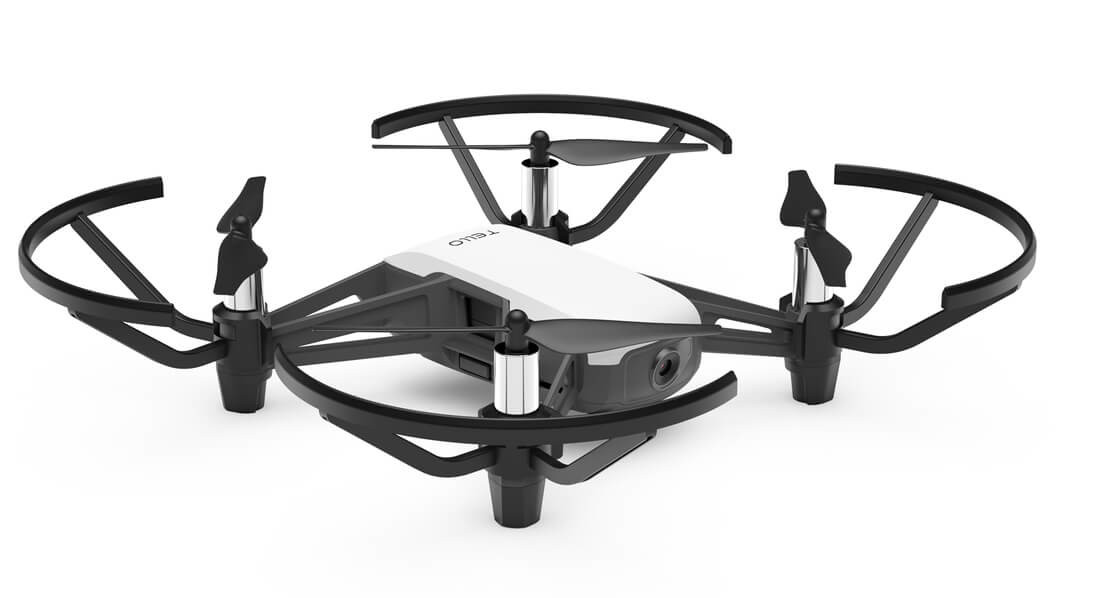
\includegraphics[width=10cm]{./Obrazy/dji-tello.jpg}
  \caption{DJI Tello}
  \source{\myurl{https://store.dji.com}}
  \end{figure}

W swojej ofercie DJI ma również dostępnego drona \textit{DJI Mini SE}, który również korzysta z technologii WiFi, ale w swoim wyposażaniu posiada dedykowany do niego kontroler. Taka konfiguracja pozwala na uzyskanie zasięgu do 2 km. \cite{dji-mavic-mini-se-spec}

WiFi jest także bardzo podatne na wszelkie zakłócenia, wynikające z ukształtowania terenu czy zaszumienia sieci pochodzącego z istniejących sieci domowych. Wyprodukowanie drona w tej technolgi jest najtańszą dostępną opcją, która umożliwia transmisje obrazu, jednak należy pamiętać, aby nie stawiać jej przy tym za dużych wymagań. Stanowi ono dobry punkt startowy w komunikacji bezprzewodowej bezzałogowych statków powietrznych.

\subsubsection{Lightbridge} TODO

Lightbridge to technologia od DJI, która doczekała się jej dwóch wydań. Pierwszych wzmianek o niej można doszukiwać się w 2014 r., a drugiego wydania już w 2015 roku. Jest ona zbliżona do technologii WiFi, przede wszystkim transmisja ta odbywa się na tej samej częstotliwości 2,4GHz.


Była ona kierowana głównie do dronów z wyższego pułapu cenowego, dlatego że jej produkcja była bardzo kosztowna, a koszt wynikał z tego, że producent opracował to rozwiązanie na swoim autorskim układzie scalonym i oprogramowaniu. Umożliwiło to osiągnąć duże lepsze wyniki niż transmisja po WiFi. Zasięg lotu według producenta to odległość do 5 km.


Obecnie Lightbridge nie jest już rozwijany, a producent skupił się na jego następniku, technologi OcuSync. \cite{lightbridge-dji}\cite{lightbridge2-dji}

\subsubsection{OcuSync} 
OcuSync został po raz pierwszy zademonstrowany przez producenta wraz z wydaniem drona \emph{Mavic Mini Pro}. Pierwsze wydanie tej technologi pozwalało na transmisje do 7 km na częstotliwości 2,4 GHz. Obraz mógł być przesyłany w rozdzielczości 720p i 1080p. Jakość fullHD była dostępna tylko na krótszych odległościach. Na większych dystansach gdy dostępna prędkość transmisji spadała, dron przechodził automatycznie na transmisje w 720 p. Opóźnienie było rzędu 160-170ms. A największą cechą wyróżniającą tę technologię była możliwość podłączenia jednocześnie dwóch kontrolerów i do 4 urządzeń odbiorczych.

Kolejnym krokiem było wydane wersji oznaczonej jako OcuSync 1.5, w której dodano transmisję również na częstotliwości 5 Ghz. Zmniejszono także opóźnienia w transmisji. Dodatkowo technologia umożliwiał automatyczną zmianę kanałów komunikacyjnych w trakcie lotu na te najmniej obciążone. W pierwszej wersji kanał
transmisji można było wybrać tylko przed startem bezzałogowego statku powietrznego.\cite{ocusync-yt}


\begin{figure}[!ht]
  \centering
  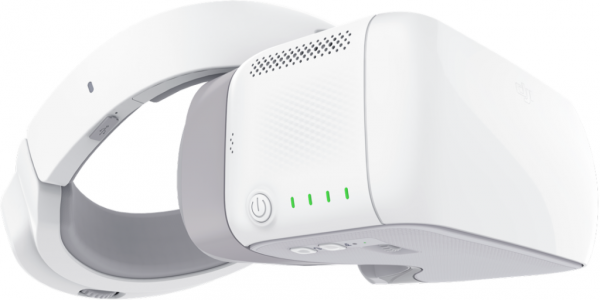
\includegraphics[width=8cm]{./Obrazy/dji-google.png}
  \caption{Pierwsza wersja gogli do FPV od DJI}
  \source{\myurl{https://u.cyfrowe.pl/600x0/2/7/2_732250420.png}}
  \end{figure}
  

\begin{figure}[!ht]
  \centering
  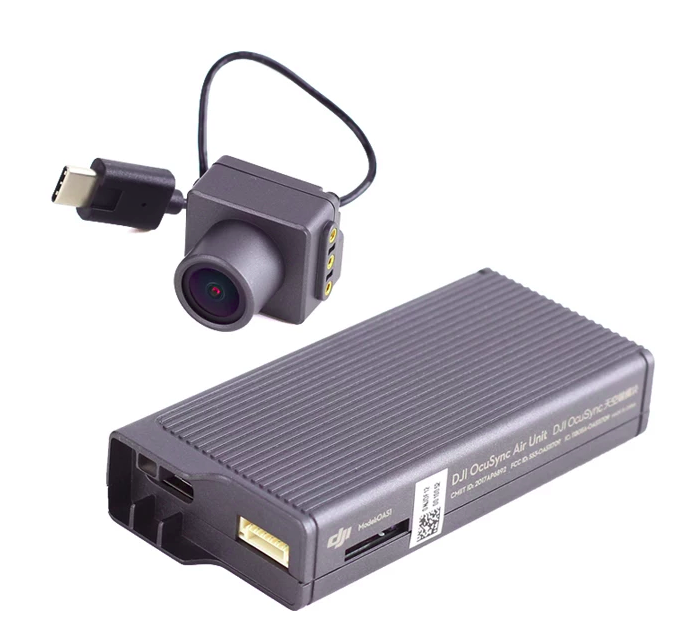
\includegraphics[width=8cm]{./Obrazy/dji-air-unit.png}
  \caption{Dji OcuSync Air Unit}
  \source{\myurl{https://store.dji.com}}
  \end{figure}

Wraz z wydaniem nowej wersji zaprezentowano \textit{gogle DJI} przeznaczone do transmisji obrazu w trybie FPV (ang. first person view, widok pierwszo-osobowy) i również \textit{OcuSync Aircraft System}, czyli zintegrowanego systemu umożliwiającego sterowanie i transmisji obrazu z wykorzystaniem tej technologi w dronach i pojazdach DIY.

Producent w trakcie swojej historii doprowadził do pewnych nieścisłości. Pomimo że dron \textit{Phantom 4 pro v 2.0} korzystał teoretycznie z najnowszej wersji OcuSync, nie posiadał on możliwości zmiany kanałów transmisji w trakcie lotu, a opóźnienie zależało też od tego, czy korzystano z kontrolera dołączonego do zestawu, czy jego droższej, lepiej wyposażonej wersji: \textit{DJI RC Plus}.
  

\begin{figure}[!ht]
  \centering
  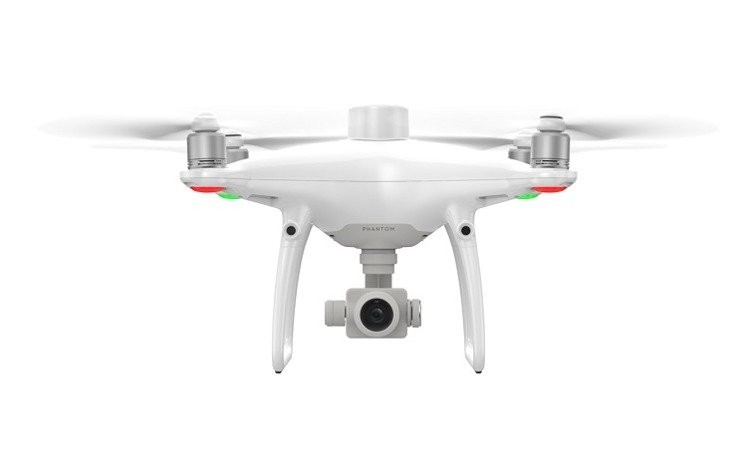
\includegraphics[width=8cm]{./Obrazy/dji-phantom-v2.jpg}
  \caption{DJI Phantom v2.0}
  \source{\myurl{https://store.dji.com}}
  \end{figure}
  

\begin{figure}[!ht]
  \centering
  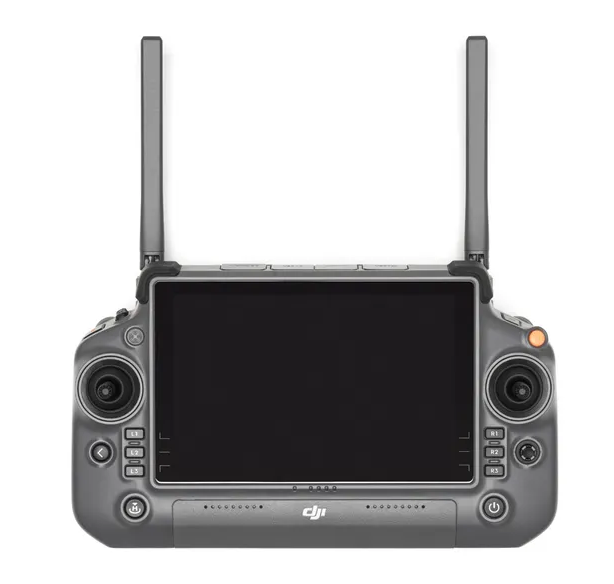
\includegraphics[width=8cm]{./Obrazy/dji-rc-plus.png}
  \caption{DJI RC plus}
  \source{\myurl{https://store.dji.com}}
  \end{figure}
  

Wersja 2.0 wprowadziła dalsze ulepszenia, m.in. kontorlowanie dronów na jeszcze większe dystanse i z jeszcze mniejszymi opóźnieniami, a także kompatybilność wsteczną po aktualizacji oprogramowania.

\newpage
\subsubsection{FHSS i  OFDM}

Zarówno Lightbridge, jak i OcuSync używają szyfrowanej modulacji OFDM (ang. Orthogonal Frequency-Division Multiplexing, zwielokrotnianie z ortogonalnym podziałem częstotliwości)) dla transmisji obrazu i z formy FHSS (ang. Frequency-Hopping Spread Spectrum) dla transmisji sygnałów sterowania. Kanał dla transmisji obrazu nie zmienia się w trakcie całego lotu, pod warunkiem, że nie następują zakłócenia, albo użytkownik nie ustawi ręcznie innej częstotliwości. Z kolei metoda FHSS "skacze" po częstotliwościach w całym dostępnym widmie, w tym nawet w pasmie przeznaczonym do transmisji obrazu.\cite{FHSS-wiki} \cite{OFDM-wiki}

\begin{figure}[!htbp]
\centering
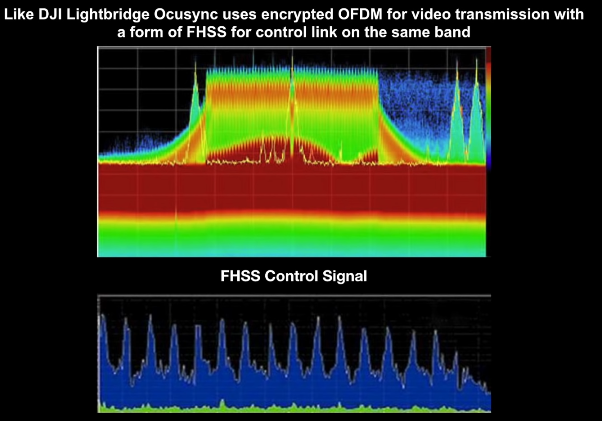
\includegraphics[width=14cm]{./Obrazy/ocusync_spectrum_1.png}
\caption{Widmo OFDM i FHSS}
\source{\myurl{https://www.youtube.com/watch?v=gfqcSv9sR0A}}
\end{figure}

\begin{figure}[!htbp]
\centering
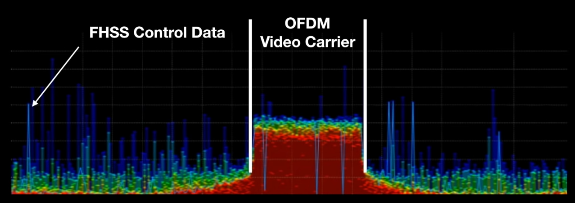
\includegraphics[width=14cm]{./Obrazy/ocusync_spectrum_2.png}
\caption{Widmo OcuSync z zaznaczoną modulacja FHSS i OFDM}
\source{\myurl{https://www.youtube.com/watch?v=gfqcSv9sR0A}}
\end{figure}


\begin{figure}[!htbp]
\centering
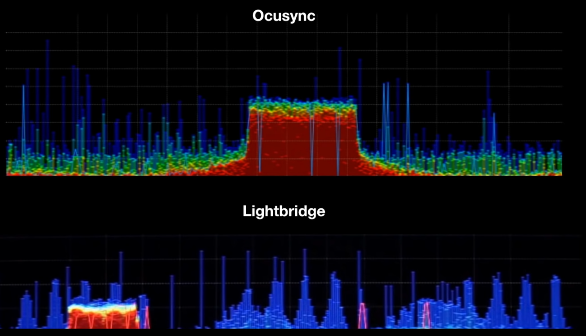
\includegraphics[width=14cm]{./Obrazy/ocusync_vs_lightbridge.png}
\caption{Porównanie widma OcuSync i Lightbridge}
\source{\myurl{https://www.youtube.com/watch?v=gfqcSv9sR0A}}v
\end{figure}

\newpage

\subsubsection{Przewaga OcuSync nad Lightbridge}
OcuSync stało się główną technologią rozwijaną przez DJI. Producent wykorzystuje układy scalone przeznaczone do komunikacji WiFi. Wytwarza na nie swoje oprogramowania, która można bez problemu aktualizować. Lightbridge nie miał takiej możliwości, a w dodatku komunikacji opierała się wyłącznie na paśmie 2,4GHz. Nowe procesory w układach WiFi dzięki coraz większej częstotliwości pracy zapewniły osiąganie tych samych efektów, co DJI uzyskiwał za pomocą autorskich układów scalonych, bez dodatkowego kosztu wynikającego z produkcji.

\subsection{Kontrolowanie BSP za pomocą API dostarczaonego od producenta}
Przeszukując internet w poszukiwaniu bezzałogowych statków powietrznych umożliwiających ich sterowanie za pomocą API od producenta, można napotkać głównie rozwiązania od DJI. Wszystkie pozostałe rozwiązania nie działają na gotowych dronach, a na oprogramowaniu przeznaczonym do wgrania na wybranych jednostkach do sterowania modelami RC.

Najpopularniejszym tego rozwiązaniem jest ArduPilot, czyli pakiet oprogramowania nawigacyjnego działającego w pojeździe wraz z oprogramowaniem sterującym stacją naziemną.

\subsubsection{DJI SDK}
DJI dostarcza do swoich produktów następujące interfejsy API:
\begin{itemize}
  \item \textbf{App Dev.} - interfejsy API przeznaczone do sterowania dronem z poziomu stacji bazowej, kontroler stanowi interfejs pośredniczący między aplikacją wykorzystującą SDK a dronem powietrznym:\begin{enumerate}
    \item \textbf{Mobile SDK} - SDK przeznaczona na platformę iOS i Android. Aplikacja na smartfon za pomocą kabla USB podłączonego do kontrolera statku powietrznego realizuje zaprogramowaną logikę działania.
    \item \textbf{UX SDK} - to Mobile SDK rozszerzony o elementy interfejsu użytkownika, co przyspiesza znacznie proces tworzenia oprogramowania.
    \item \textbf{Windows SDK} - SDK umożliwiające wydawanie aplikacji na systemach operacyjnych Windows. 
  \end{enumerate}
  \item \textbf{Payload Dev.} - interfejsy API przeznaczone do nadawania logiki działania drona na poziomie samego drona, dzięki temu po utracie zasięgu może ona dalej funkcjonować. Opcja dostępna dla najdroższych wersji dronów DJI, które można dostosowywać do swoich wymagań za pomocą odpowiednich rozszerzeń, np. kamery termowizyjnej\begin{enumerate}
    \item \textbf{Payload SDK} - zestaw narzędzi programistycznych umożliwiających tworzenie oprogramowania do rozszerzeń, które mogą być montowane na dronach DJI. 
    \item \textbf{Onboard SDK} - otwarto-źródłowe API umożliwiające bezpośrednią komunikację z wybranymi dronami i kontrolerami za pomocą interfejsu szeregowego.
  \end{enumerate}
\end{itemize}

\newpage
\section{Projekt mobilnego systemu zarządzania i sterowania BSP}
\subsection{Wymagania funkcjonalne}
text
\subsection{Wymagania pozafunkcjonalne}
text
\subsection{Stos technologiczny}
text
\subsubsection{Java}
text
\subsubsection{Kotlin}
text
\subsubsection{DJI Mobile SDK}
text
\subsubsection{Lombook}
text
\subsubsection{Springboot}
text
\subsubsection{Android}
text
\subsection{Uzasadnienie warstwy pośredniczącej}
text
\subsection{Wysokopoziomowy diagram systemu}
text
\subsection{Diagram komponentów}
text
\subsection{Diagram klas i sekwencji}
text
\subsubsection{Gradle}
text
\subsection{Wykorzystane urządzenia}
text

\newpage
\section{Implementacja systemu}

\newpage
\section{Testy systemu oraz prezentacja użycia na wybranym case study}
TODO

\subsection{Testy jednostkowe TODO}
W kontekście testowania oprogramowania na platformie andorid można wyróźnić dwa rodzaje testów jednostkowych.
\begin{itemize} 
  \item \textbf{androidTest} - Testy, które są uruchamiane na rzeczywistych lub wirtualnych urządzeniach z systemem Androdi. Obejmują one m.in. test integracyjne i end-to-end, w których samo JVM nie może sprawdzić działania kodu. W ramach tego rozdzaju testów przetestowano serwisy odpowiedzialne za komunikacje za pomocą MQTT, ponieważ są to operacje asynchroniczne, a biblioteka która jest wykrozysytwana potrzbuje w konstruktorze do swojego działania kontekstu aplikacji android (klasa /textit{android.content.Context}) .
  \item \textbf{test} - Klasyczne testy jednostkowe, które mogą być uruchamiane w ramach JVM na loklanej masyznie. W ramach tych testów przetestowano m.in. mapowanie opiektów JSON na klasy DTO przysyłancyh komend (klasa \textit{pl.edu.wat.droman.data.model.command.Command})
\end{itemize}

\subsubsection{Testowanie MqttService}
Klasa \textit{pl.edu.wat.droman.data.service.MqttService} odpowiada za zarządzania obsługowywanymi Topic-ami MQTT. Zwraca ona dla podanej scieżki obiekt klasy \textit{pl.edu.wat.droman.data.service.MqttService.Topic} na którym można wykonywać opcje publikowania i subkrybowania wiadomości MQTT. Ponieważ zwraca ona obiekty za pomoca klasy /textit{androidx.lifecycle.LiveData} operacje te są wykonywane z kontekstem aplikacji. Dodatkowo w całym procesie wykorzysytywany jest do tego serwer MQTT, którego parametry logowania i adresu są pobierane z pliku konfiguracyjengo gradle, który jest przechowywany na loklanej maszynie, dzięki temu hasła nie są przechowywane razem z kodem na repozytorium Git.

\begin{lstlisting}[language=Kotlin, caption=Inicjalizowanie wartosci w klasie przed uruchominiem poszczególnych testów\label{TbECMont}]
  @Before
    fun init() {
        appContext = InstrumentationRegistry.getInstrumentation().targetContext

        val metadata: Bundle = appContext.packageManager.getApplicationInfo(
            appContext.packageName,
            PackageManager.GET_META_DATA
        ).metaData

        password = metadata.getString("mosquitto.password")!!
        user = metadata.getString("mosquitto.user")!!
        uri = "tcp://" + metadata.getString("mosquitto.ip")
        mqttService = MqttService(appContext, MqttCredentials(uri, clientID, user, password))
    }
\end{lstlisting}

\begin{lstlisting}[language=Kotlin, caption=Test publikowania danych za pomocą Mqtt \label{TbECMont}]

  @Test
  fun publish() = runBlocking {
      //given

      val message = "message:" + UUID.randomUUID()
      val topicVal = "/test"

      //then
      val topic = mqttService.getTopic(topicVal)
      val res = topic.publish(message)

      //except
      Assert.assertTrue(res.isSuccess)
  }

\end{lstlisting}


\begin{lstlisting}[language=Kotlin, caption=Test pobierania danych za pomocą Mqtt \label{TbECMont}]
  @Test
  fun getData() {
      //given

      val message = "message:" + UUID.randomUUID()
      val message2 = "message:" + UUID.randomUUID()
      val topicVal = "/test"

      //then
      val topic = mqttService.getTopic(topicVal)
      runBlocking {
          topic.subscribe()
          topic.publish(message)
      }

      //except
      Assert.assertEquals(message, topic.getData().getOrAwaitValue(time = 5).toString())
      
      //then
      runBlocking {
          topic.publish(message)
      }
      
      //except
      Assert.assertEquals(message, topic.getData().getOrAwaitValue(time = 5).toString())
  }
\end{lstlisting}





\begin{figure}[!ht]
  \centering
  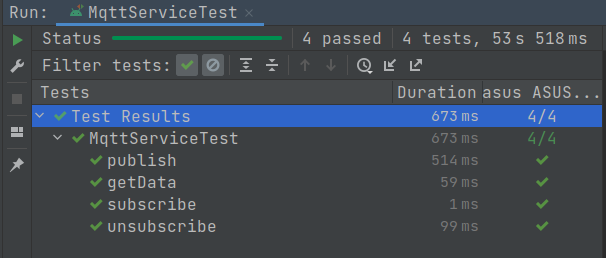
\includegraphics[width=12cm]{./Obrazy/MqttTestResult.png}
  \caption{Wynik testów MqttRepository}
  \source{Własne}
  \end{figure}

\subsubsection{Testowanie CommandFactory}


\begin{lstlisting}[language=Kotlin, caption=Test tworzenia komendy \textit{UploadWaypointCommand} za pomocą \textit{CommandFactory} \label{TbECMont}]
  @Test
  fun testMappingToUploadMissionCommand() {
      //given
      val commandFactory = CommandFactory()
      val missionValue = "{\n" +
              "            \"type\": \"upload_waypoint_mission\",\n" +
              "            \"finished_action\": \"NO_ACTION\",\n" +
              "            \"auto_flight_speed\": 0.01,\n" +
              "            \"max_flight_speed\": 0.5,\n" +
              "            \"heading_mode\": \"AUTO\",\n" +
              "            \"waypoints\": [\n" +
              "                {\n" +
              "                    \"attitude\": 1.0,\n" +
              "                    \"longitude\": 1.0,\n" +
              "                    \"latitude\": 1.0\n" +
              "                },\n" +
              "                {\n" +
              "                    \"attitude\": 1.0,\n" +
              "                    \"longitude\": 1.0,\n" +
              "                    \"latitude\": 1.0\n" +
              "                },\n" +
              "                {\n" +
              "                    \"attitude\": 1.0,\n" +
              "                    \"longitude\": 1.0,\n" +
              "                    \"latitude\": 1.0\n" +
              "                }\n" +
              "            ]\n" +
              "        }"
      //then
      val command = commandFactory.from(missionValue)

      //expect
      assertNotNull(command)
      assertEquals(UploadWaypointCommand.type, command.type)
      assertEquals(UploadWaypointCommand::class.java,command.javaClass)
  }
\end{lstlisting}

\begin{lstlisting}[language=Kotlin, caption=Przykładowy test klasy MqttService \label{TbECMont}]

  @Test
  fun testMappingToFailUploadMissionCommand() {
      //given
      val commandFactory = CommandFactory()
      val missionValue = "{\"type\": \"dsadas\"}"
      //then
      val command = commandFactory.from(missionValue)

      //expect
      assertNotNull(command)
      assertEquals(UnrecognizedCommand::class.java,command.javaClass)
      assertEquals(UnrecognizedCommand.type, command.type)
  }
\end{lstlisting}

\begin{lstlisting}[language=Kotlin, caption=Przykładowy test klasy MqttService \label{TbECMont}]

  @Test
  fun testMappingToTakeOffCommand() {
      //given
      val commandFactory = CommandFactory()
      val missionValue = "{\"type\": \"take_off\"}"
      //then
      val command = commandFactory.from(missionValue)

      //expect
      assertNotNull(command)
      assertEquals(TakeOffCommand::class.java,command.javaClass)
      assertEquals(TakeOffCommand.type, command.type)
  }
\end{lstlisting}


\subsection{Scenariusz testowy autonomicznego lotu patrolowego}

\newpage
\section{TMP}

\subsection{Tytuł podrozdziału}
W procesie dyplomowania tekst pracy jest przetwarzany elektronicznie za pośrednictwem systemów USOS APD (Archiwum Prac Dyplomowych) oraz JSA (Jednolity System Antyplagiatowy). Plik pracy zapisany w formacie ,,pdf'' winien mieć nazwę nadana wg schematu: \textit{,,WAT, myślnik, numer indeksu studenta, myślnik, data wysłania w formacie dd-mm-rrrr''}, np. \textit{,,WAT-12345-01.05.2021.pdf''}. Plik umieszczany jest w systemie USOS APD poprzez indywidualne konto Dyplomanta.

Do pracy można załączyć dodatkowe pliki w formacie ,,docx''/,,pdf''.`'
W przypadku innych formatów (w tym „zip”) , należy je zapisać na płycie CD/DVD, opisanej trwale (niezmywalnym mazakiem) następująco: skrót nazwy uczelni, nazwa wydziału, kierunek studiów, specjalność, numer albumu studenta, imię i nazwisko studenta, temat pracy dyplomowej, własnoręczny podpis studenta. 

\subsection{Tytuł podrozdziału}

W tekście pracy kolejne wątki tematyczne należy oddzielać poprzez wcięciami akapitowe. W strukturze pracy zalecane jest:
\begin{itemize} 
    \item w przypadku wprowadzenia podrozdziałów wyróżnienie co najmniej dwóch na danym poziomie zagłębienia.
\end{itemize}

Praca powinna zawierać oryginalny tekst. W przypadku cytowania należy stosować przypisy dolne. W przypadku odwołania do literatury lub źródeł internetowych należy wstawiać hiperłącza do odpowiednich pozycji z bibliografii, np. [1].
 
Wszystkie skróty w pracy przy pierwszym ich użyciu powinny być rozwinięte (wyjaśnione). Pojedyncze litery z końca wierszy powinny być przeniesione na początek kolejnych wierszy poprzez wprowadzenie tzw. ,,twardej spacji'' pomiędzy tą literą a kolejnym wyrazem (np. w edytorze Microsoft Word poprzez kombinację klawiszy Ctrl+Shift+Spacja).

Pracę mogą kończyć spisy rysunków i tabel – zalecane jest ich wprowadzenie w przypadku wystąpienia dużej liczby rysunków lub tabel w tekście pracy (powyżej 10). Praca może być uzupełniona załącznikami. W przypadku braku w pracy spisów rysunków i tabel lub załączników należy usunąć je ze struktury pracy oraz spisu treści.

Dla tekstu, tytułów, podpisów należy stosować style Wydziału (docx) lub zdefiniowane w~tym szablonie.\\
Układ marginesów i numerów stron przewidziany jest do wydruku dwustronnego.\\
Wydruk pracy nie jest wymagany.


Tabele i rysunki należy wyśrodkować. Dla podpisów stosowane są style Wydziału (docx) lub otoczenie table i tabular oraz figure (LaTeX):
\begin{itemize}
    \item Nazwa tabeli umieszczona ponad tabelą;
    \item Podpis rysunku umieszczony pod rysunkiem;
    \item Źródło rysunku lub danych w tabeli pod tabelą/rysunkiem.
\end{itemize}
Numeracja tabel i rysunków powinna być ciągła i automatyczna w całej pracy.
\begin{table}[H]
    \caption{Nazwa tabeli}
    \label{tab1}
    \begin{center}
        \begin{tabular}{|c|c|c|c|}
                \hline
                \textbf{Lp}     & \textbf{Kolumna 1}    & \textbf{Kolumna 2}    & \textbf{Kolumna 3}    \\ \hline
                1.              & Zawartość tabeli      & Zawartość tabeli      & Zawartość tabeli   \\ \hline
        \end{tabular}
    \end{center}
    \source{Badania własne. Jeżeli dane pochodzą z literatury lub zasobów sieci Internet, należy podać ich źródło. W~innym przypadku można podać: Badania własne.}
\end{table}

Dla wzorów zaleca się stosować wyśrodkowanie. Numerację automatyczną ciągłą w~całej pracy należy wyrównać do prawej strony – przykład poniżej:
\begin{equation}
    \label{eq1}
    \displaystyle \sum_{j=0}^{n}a_{ij} \leq 1, i = \overline{1, n}
\end{equation}

Kod źródłowy oraz algorytmy umieszcza się w tabelach dwukolumnowych (docx), lub otoczenia lstlisting i algorithm (LaTeX), z numeracją wierszy w pierwszej kolumnie:
\begin{itemize}
    \item Tekst w tabeli kodu źródłowego: czcionka Courier New 11 pkt., wyjustowany do lewej;
    \item Nazwa kodu źródłowego umieszczona ponad kodem;
    \item Nazwa algorytmu umieszczona ponad algorytmem;
    \item Źródło kodu lub algorytmu poniżej.
\end{itemize}

\begin{lstlisting}[language=Verilog, caption=Nazwa kodu źródłowego \label{TbECMont}]
    int silnia (int a)
    {
        return (a == 1) ? a : a * silnia(a-1);
    }
\end{lstlisting}
\source{Badania własne. Jeżeli dane pochodzą z literatury lub zasobów sieci Internet, należy podać ich źródło. W~innym przypadku można podać: Badania własne.}

\begin{algorithm}[H]
    \caption{Nazwa algorytmu}
    \label{alg_nazwa}
    \hrule
\begin{verbnobox}[\verbarg]
wczytaj(n)
inicjuj tab[1..n]
dla i ← 1 do n powtarzaj
    wczytaj tab[i]
dla i ← 1 do n powtarzaj
    dla j ← i + 1 do n powtarzaj
        jeżeli tab[j] < tab[j - 1] to
            pom ← tab[j]
            tab[j] ← tab[j - 1]
            tab[j - 1] ← pom
dla i ← 1 do n powtarzaj
    wypisz(tab[i])
\end{verbnobox}
    \hrule
    \source{Badania własne. Jeżeli dane pochodzą z literatury lub zasobów sieci Internet, należy podać ich źródło. W~innym przypadku można podać: Badania własne.}
\end{algorithm}

%Odniesienie do rysunku \ref{rys01.png}\\
%
%Odniesienie do tabeli \ref{tab1}\\
%
%Odniesienie do wzoru \ref{eq1}\\
%
%Odniesienie do algorytmu \ref{alg_nazwa}\\
%
%Odniesienie do kodu \ref{TbECMont}\\
%
%Odniesienie do bibliografii \cite{pos3}

\clearpage \section*{Podsumowanie} \addcontentsline{toc}{section}{Podsumowanie}

% Podsumowanie powinno korespondować z tematem i założonymi celami pracy. Zaleca się, aby zawierało syntetyczne podsumowanie wyników z odniesieniem do stopnia realizacji oraz wskazaniem najważniejszych osiągnięć i słabszych stron pracy. Może również obejmować omówienie podobieństw i różnic między uzyskanymi a publikowanymi wynikami innych autorów. Ponadto, winno przedstawiać dalsze interesujące kierunki rozwoju pracy.

\clearpage \begin{thebibliography}{999}
\addcontentsline{toc}{section}{\refname}

\bibitem{dron-ibuk}
Sarah E. Kreps
\bibTitle{Drony. Wprowadzenie Technologie Zastosowania}
Wydawnictwo Naukowe PWN, Warszawa, 2019;

\bibitem{arton-kelsey}
A. Kelsey
\bibTitle{Flying Robots 101: Everthing You Need to Know about Drones}, Popular Science, TODO TOM, TODO STRONY, 08-03-2013

\bibitem{NB-IoT_vs_Lora}
\bibTitle{NB-IoT vs Lora}
\myurl{https://ubidots.com/blog/lorawan-vs-nb-iot/\#lorawan-vs-nb-iot-a-quick-overview} [dostęp: 20-04-2022];

\bibitem{m2m-web}
\bibTitle{machine-to-machine (M2M)}
\myurl{https://www.techtarget.com/iotagenda/definition/machine-to-machine-M2M} [dostęp: 20-04-2022];

\bibitem{LPWA-wiki}
\bibTitle{LPWA wikipedia}
\myurl{https://pl.wikipedia.org/wiki/LPWAN} [dostęp: 20-04-2022];

\bibitem{LoRa-article}
\bibTitle{LoRa Technology - An Overview, IEEE, 2018}
\myurl{https://ieeexplore.ieee.org/document/8474715} [dostęp: 20-04-2022];


\bibitem{yuneec-wiki}
\bibTitle{Wikipedia: Yuneec International}
\myurl{https://en.wikipedia.org/wiki/Yuneec_International} [dostęp: 25-04-2022];

\bibitem{nbiot-article}
\bibTitle{On the Performance of Narrow-band Internet of
Things (NB-IoT) for Delay-tolerant Services, IEEE, 2019}
\myurl{https://ieeexplore.ieee.org/document/8768871} [dostęp: 20-04-2022];

\bibitem{dji-wiki}
\bibTitle{Wikipedia: SZ DJI Technology Co., Ltd.},
\myurl{https://en.wikipedia.org/wiki/DJI} [dostęp: 20-04-2022];

\bibitem{queen-bee}
\bibTitle{De Havilland DH-82 "Tiger Moth" ("Queen Bee"), 1931},
\myurl{http://www.samolotypolskie.pl/samoloty/782/126/De-Havilland-DH-82-Tiger-Moth-Queen-Bee} [dostęp: 22-04-2022];

\bibitem{dji-market-share}
\bibTitle{DJI market share: here’s exactly how rapidly it has grown in just a few years},
\myurl{https://www.thedronegirl.com/2018/09/18/dji-market-share/} [dostęp: 22404-2022];

\bibitem{fotografia-drony-ukraina}
\bibTitle{Wojna w Ukrainie: Pasjonaci dronów namierzają rosyjskie wojska},
\myurl{https://fotoblogia.pl/17711,wojna-w-ukrainie-pasjonaci-dronow-namierzaja-rosyjskie-wojska} [dostęp: 22-04-2022];

\bibitem{bayraktar-chip}
\bibTitle{Tureckie drony na Ukrainie pokazały wojnę przyszłości. Bayraktar TB2 wyrządzają ogromne szkody},
\myurl{https://www.chip.pl/2022/03/tureckie-drony-w-ukrainie-pokazaly-wojne-przyszlosci-bayraktar-tb2-wyrzadzaja-ogromne-szkody/} [dostęp: 22-04-2022];

\bibitem{bayraktar-pap}
\bibTitle{Zaskakująca skuteczność Bayraktarów. Ekspert o rosnącej roli dronów w wojnie},
\myurl{https://www.pap.pl/aktualnosci/news\%2C1129159\%2Czaskakujaca-skutecznosc-bayraktarow-ekspert-o-rosnacej-roli-dronow-w} [dostęp: 22-04-2022];

\bibitem{dji-mavic-mini-se-spec}
\bibTitle{DJI Mavic Mini SE},
\myurl{https://www.dji.com/pl/mini-se?site=brandsite&from=nav} [dostęp: 20-04-2022];

\bibitem{dji-store}
\bibTitle{DJI store},
\myurl{https://store.dji.com} [dostęp: 20-04-2022];

\bibitem{lightbridge-dji}
\bibTitle{DJI Lightbridge},
\myurl{https://www.dji.com/pl/dji-lightbridge/info} [dostęp: 20-04-2022];

\bibitem{lightbridge2-dji}
\bibTitle{DJI Lightbridge2},
\myurl{https://www.dji.com/pl/lightbridge-2/info\#specs} [dostęp: 20-04-2022];

\bibitem{OFDM-wiki}
\bibTitle{Wikipedia: OFDM},
\myurl{https://pl.wikipedia.org/wiki/OFDM} [dostęp: 20-04-2022];

\bibitem{firebee-wiki}
\bibTitle{Wikipedia: Ryan Model 147 Lightning Bug},
\myurl{https://en.wikipedia.org/wiki/Ryan_Model_147} [dostęp: 22-04-2022];

\bibitem{predator-wiki}
\bibTitle{Wikipedia: MQ-1 Predator},
\myurl{https://en.wikipedia.org/wiki/General_Atomics_MQ-1_Predator} [dostęp: 22-04-2022];

\bibitem{baykar-wiki}
\bibTitle{Wikipedia: Baykar},
\myurl{https://en.wikipedia.org/wiki/Baykar} [dostęp: 22-04-2022];

\bibitem{FHSS-wiki}
\bibTitle{Wikipedia: FHSS},
\myurl{https://pl.wikipedia.org/wiki/FHSS} [dostęp: 20-04-2022];

\bibitem{ocusync-yt}
\bibTitle{DJI Mavic 2 - Ocusync 2.0 What is it \& What's Compatible ? + How is it different from Lightbridge},
\myurl{https://www.youtube.com/watch?v=gfqcSv9sR0A} [dostęp: 20-04-2022];

\bibitem{dji-gogle}
\bibTitle{DJI Gogle},
\myurl{https://u.cyfrowe.pl/600x0/2/7/2_732250420.png} [dostęp: 20-04-2022];

\bibitem{konkurs-mon}
\bibTitle{Konkurs MON na bezzałogowe sytemy powietrzne, lądowe, morskie},
\myurl{https://www.wojsko-polskie.pl/wat/articles/aktualnosci-w/konkurs-mon-na-bezzalogowe-systemy-powietrzne-ladowe-i-morskie/} [dostęp: 21-04-2022];

\bibitem{wiki-gaas}
\bibTitle{Wikipedia: General Atomics Aeronautical Systems},
\myurl{https://en.wikipedia.org/wiki/General_Atomics_Aeronautical_Systems} [dostęp: 26-04-2022];

\bibitem{gd-about}
\bibTitle{General Dynamics: Our history},
\myurl{https://www.gd.com/about-gd/our-history} [dostęp: 26-04-2022];

\bibitem{pansa-lot-medyczny}
\bibTitle{PANSA: Ruszają regularne loty transportowe BSP},
\myurl{https://www.pansa.pl/ruszaja-regularne-loty-transportowe-bsp/} [dostęp: 28-04-2022];

\bibitem{topr-dron}
\bibTitle{Akcja TOPR dron dostarczył koce i ogrzewacze},
\myurl{http://www.swiatdronow.pl/akcja-topr-dron-dostarczyl-koce-i-ogrzewacze/} [dostęp: 28-04-2022];

\bibitem{snowbrains-drone}
\bibTitle{Drones to the Rescue? How Drones are Changing the Landscape of High Mountain Rescue Efforts},
\myurl{https://snowbrains.com/drones-to-the-rescue-how-drones-are-changing-the-landscape-of-high-mountain-rescue-efforts/} [dostęp: 29-04-2022];

\bibitem{bbc-drone-rescue}
\bibTitle{Drones guide rescuers to hunter lost in North Carolina woods, officials say},
\myurl{https://www.newsobserver.com/news/state/north-carolina/article260714992.html/} [dostęp: 29-04-2022]; 

\bibitem{dron-lawa-pogoda}
\bibTitle{Wleciał dronem do wnętrza wulkanu na Islandii. Ostatnie sekundy nagrania jeżą włosy na głowie [WIDEO]},
\myurl{https://www.twojapogoda.pl/wiadomosc/2021-06-02/wlecial-dronem-do-wnetrza-wulkanu-na-islandii-ostatnie-sekundy-nagrania-jeza-wlosy-na-glowie-wideo/} [dostęp: 29-04-2022]; 

\bibitem{washingtonpost-drone-movie}
\bibTitle{It’s a bird! It’s a plane! It’s a drone that makes movies!},
\myurl{https://www.washingtonpost.com/news/the-switch/wp/2013/08/15/its-a-bird-its-a-plane-its-a-drone-that-makes-movies/} [dostęp: 29-04-2022]; 

\bibitem{how-to-build-drone}
\bibTitle{How to Build a Drone: Construct Your Drone from Scratch},
\myurl{https://www.mydronelab.com/blog/how-to-build-a-drone.html} [dostęp: 29-04-2022]; 

\bibitem{drone-transport}
\bibTitle{Drone Delivery Was Supposed to be the Future. What Went Wrong?},
\myurl{https://www.youtube.com/watch?v=J-M98KLgaUU} [dostęp: 29-04-2022]; 



\bibitem{sosnowiec-drone}
\bibTitle{Drony przetransportują sprzęt medyczny nad Sosnowcem. Przed nami spotkanie z mieszkańcami},
\myurl{https://sosnowiec.naszemiasto.pl/drony-przetransportuja-sprzet-medyczny-nad-sosnowcem-przed/ar/c1-8493233} [dostęp: 29-04-2022]; 



 

\end{thebibliography}

\clearpage

\listoffigures
\addcontentsline{toc}{section}{Spis rysunków}

\listoftables
\addcontentsline{toc}{section}{Spis tabel}

\clearpage \section*{Załączniki}
\addcontentsline{toc}{section}{Załączniki}
\begin{enumerate}
    \item Płyta CD/DVD zawierająca:
    \begin{enumerate}
        \item Prezentację wyników pracy dyplomowej
        \item Kody źródłowe oprogramowania
        \item Biblioteki programowe niezbędne do zbudowania i uruchomienia oprogramowania
        \item ...
    \end{enumerate}
    \item ...
\end{enumerate}

\end{document}